\chapter{Generalized frequency division multiplexing multiple input multiple output}\label{sec:GFDMMIMO}
\section{System model}\label{part:SM1}
In this chapter we assume the GFDM MIMO system  the flat-frequency channel\cite{Book25}\cite{Book29} in that case the system is explained in the 
\eqref{mim_1} equation with channel model a identity matrix without multipath propagation.
\begin{align}
\mathbf{Y}=\mathbf{HZ}+\mathbf{N}
\label{mim_1}
\end{align}
\begin{align*}
\mathbf{H}\in\compl^{M_r\times M_t}
\mathbf{Z}\in\compl^{M_t\times T}
\mathbf{N,Y}\in\compl^{M_r\times T}
\end{align*}
%\subsection{MIMO model}
The GFDM system in MIMO AWGN case can be explained with the PARATUCK2 third order model. The difference between the SISO and MIMO case is significant\cite{Book29}, but PARATUCK2 model allow to extend  matrices to define the MIMO case inside of the same mathematical structure. The received data should have certain dimensionality $\mathbf{Y}\in\compl^{M_r\times T}$
The symbol matrix $\mathbf{S}$ from the SISO system become three dimensional tensor $\mathcal{S}\in\compl^{F\times T_s\times M_t}$ in the MIMO case. Additional dimension corresponds to the symbols which is transmitted from the different transmit antennas. The PARATUCK2 does not allow using tensors in the model. To overcome this constraint we transform the $\mathcal{X}$ into the stacked slices for each $m_t$ \eqref{mimo_1}.
\begin{align}
\mathbf{S}=\begin{bmatrix}
\mathcal{S}_{:,:,1}\\
\mathcal{S}_{:,:,2}\\
\vdots \\
\mathcal{S}_{:,:,M_t}\\
\end{bmatrix} \label{mimo_1}
\end{align}
\begin{align*}
\mathcal{S}\in\compl^{F\times T_s\times M_t}
\mathbf{S}\in\compl^{F\cdot M_t\times T_s}
\end{align*}
The $C^{[b]}$ matrix stay the same as in the SISO model and does not change with increasing of the transmit antennas \eqref{mim_2}. In the columns of the matrix stays the same time mixing filter which doesn't change from the number of the transmit and receive antennas. From the right hand side the $\mathbf{S}$ does not change and have number of the columns $T_s$ which also satisfy the model.
\begin{align}
\mathbf{C}^{[b]}\in\compl^{T\times T_s}
\label{mim_2}
\end{align}
The connection array $\mathbf{b}$ stay the same as in the SISO case \eqref{mimo_3}. The necessary assumption for this is linear time invariant transmission channel in terms of the one transmission block. We fill the $\mathbf{b}$ array with all-ones as in the SISO case.
\begin{align}
\mathbf{b}=\mathbf{1}_{T_s\times 1} \label{mimo_3}
\end{align}
\begin{align*}
\mathbf{b} \in\compl^{T_s\times 1} 
\end{align*}
The $\mathbf{C}^{[a]}$ matrix in the MIMO case is changed \eqref{mimo_4}. Define this matrix in the MIMO case as $\mathbf{C}^{[a]'}$. Regarding to the $\mathbf{S}$ matrix, dimensions of the $\mathbf{C}^{[a]'}$ should be $T \times F\cdot M_t$. In comparison with the SISO model, in the MIMO case $\mathbf{S}$ should be multiplied with the $\mathbf{C}^{[a]}$ matrices. The new $\mathbf{C}^{[a]'}$ become stacked repeated version of the $\mathbf{C}^{[a]}$ matrix \eqref{mimo_5}. Hadamard product between $\mathbf{S}$ and the $\mathbf{C}^{[a]'}$ become simple explanation of the sub-carrier modulation of the each sub-frequency at the each transmitter antenna. Sub-carriers in the each transmit antennas is equal, so $\mathbf{C}^{[a]}$ matrices for each $m_t$ is also equal.
\begin{align}
\mathbf{C}^{[a]'}=
\begin{bmatrix}
\mathbf{C}^{[a]}& \mathbf{C}^{[a]}& \cdots &\mathbf{C}^{[a]}\\
\end{bmatrix} \in\compl^{T\times M_t\cdot F} \label{mimo_4}
\end{align}
\begin{align}
\mathbf{C}^{[a]'}=(\mathbf{1}_{1\times M_t} \otimes \mathbf{C}^{[a]}) \in \compl^{  T\times M_t\cdot F} \label{mimo_5}
\end{align}
The $\mathbf{a}$ array become the matrix and connect each $m_r$ antenna with the each $m_t$ transmit antenna and include every sub-carrier coefficient\eqref{mimo_6}. Define sub-carrier coefficients as the $\mathcal{A}$ tensor with coefficients for each $m_r,m_t,f$. In the PARATUCK2 model $\mathbf{A}$ is the matrix, we must define the $\mathcal{A}$ as the matrix which will sum for every transmit antenna sub-carrier frequency with corresponding sub-carrier coefficient\eqref{mimo_7}. Regarding to the $\mathbf{S}$ matrix, symbols is located sequentially for each sub-carrier at each transmit antenna. The $\mathbf{A}$ dimension is $M_r \times F\cdot M_t$. The first unfolding of the $\mathcal{A}$ have corresponding sub-carrier coefficients following the $\mathbf{S}$ symbols\eqref{mimo_8}. This notation multiplies each sub-carrier coefficient $\mathbf{A}$ to each symbol from the $\mathbf{S}$.
\begin{align}
\mathcal{A} \in \compl^{M_r\times F\times M_t} \label{mimo_6}
\end{align}
\begin{align}
\mathbf{A}=\mathcal{A}_{[1]} \label{mimo_7}
\end{align}
\begin{align}
\mathbf{A}\in\compl^{M_r \times F\cdot M_t} \label{mimo_8}
\end{align}
The overall model with explained matrices will be defined in the \eqref{mimo_9}. This model define the received data. All operation, which was explained in the GFDM SISO part is also applicable in the GFDM MIMO case. It should be noted that the rank of the $\mathbf{A}$ is $min(M_r,F\cdot M_t)$ in the real case number of the receive antennas is much less than sub-carriers multiplied with transmit antennas. The rank of the matrix $\mathbf{A}$ show how many transmit coefficient possible to know in the system with known transmitted symbols.
\begin{align}
\mathbf{HZ}=\mathbf{X}=\mathbf{A}\cdot (\mathbf{C}^{[a]'T} \odot (\mathbf{S}\cdot (\mathbf{C}^{[b]}\diamond \mathbf{B})^T)) \label{mimo_9}
\end{align}
\begin{align*}
\mathbf{X}\in\compl^{M_r \times T}
\mathbf{A}\in\compl^{M_r \times F\cdot M_t}
\mathbf{C}^{[a]'}\in\compl^{T \times F\cdot M_t}
\end{align*}
\begin{align*}
\mathbf{S}\in\compl^{F\cdot M_t \times T_s}
\mathbf{C}^{[b]}\in\compl^{T \times T_s}
\mathbf{B}\in\compl^{1 \times T_s}
\end{align*}

\section{Sub-carrier coefficient update approach}\label{part:SCUA}
The spectrum sensing approach is applicable in the MIMO system too. One of the important properties in the MIMO system is diversity, which frequently achieved via spatial location of the transmitter and receiver antennas\cite{Book29}. It should be noted that for different transmitter-receiver antenna pair one sub-carrier may be occupied with another system, and not. Receiver must know the $\mathbf{A}$ to know how data is transmitted. Sub-carrier coefficients update is complex task due to the time mix and multi-frequency system. The number of the unknown variables in the system for MIMO case equal to the $M_r\cdot M_t\cdot F$. Number of the equations to solve equal to the $T\cdot M_r$ for each transmission block. The transmission coefficients can be found with specially structured known symbol matrix. 
\subsection{Approximated approach}
The one way to find the matrix $\mathbf{A}$ with sub-carrier coefficients is semi-blind receiver. The number of time slots must equal to the number of the transmit antennas. The receiver may use approach from the previous chapter \ref{part:SCSSISO}. Transmitter should construct special structure of the matrix $\mathbf{S}$. For each time slot the receiver can find the $M_r\cdot F$ transmission coefficients. The transmitter must fill at least $M_t$ time slots with known symbols to find the all $\mathbf{A}$ matrix. The search algorithm for the  matrix $\mathbf{A}$ is next:
\begin{itemize}
\item Transmitter put inside the transmission block specially structured symbols. Transmitter put known to the receiver symbol row to the one transmit antenna at the each time slot. In other words the symbols are sent from each sub-carrier frequency in the certain antenna.  Transmitter repeats the same row, but from another transmit antenna at the next time slot. The transmitter repeat process $M_t$ times for each antenna. The receiver must know the   transmission order. 
\item  The receiver has transmission block with $M_t$ time slots length. The receiver uses semi-blind approach from the SISO case and assume received signal is sent from the SISO system. Semi-blind receiver approach estimates the sub-carrier coefficients for $m_t$-th transmit antenna.
\item The receiver repeats process for another time slot, and estimates the sub-carrier coefficients for another transmit antenna. The receiver repeats process $M_t$ times until estimates the all $\mathbf{A}$ matrix elements.
\end{itemize}
\subsection{MIMO model based approach}
The matrix $\mathbf{A}$ will be found with the equation \eqref{mimo_msm_4} separation  in the PARATUCK2 model. The model is written as the vectorized matrix $\mathbf{A}$ multiplication with the intermediate matrix $\mathbf{\Delta}$, as given in \eqref{mimo_msm_5}. 
\begin{align}
\mathbf{Y}=\mathbf{HZ}+\mathbf{N} \label{mimo_msm_1}
\end{align}
\begin{align}
\mathbf{HZ}=\mathbf{X}=\mathbf{A}\cdot (\mathbf{C}^{[a]'T} \odot (\mathbf{S}\cdot (\mathbf{C}^{[b]}\diamond \mathbf{b}^T)^T)) \label{mimo_msm_2}
\end{align}
\begin{align*}
\mathbf{Y,X,N}\in\compl^{M_r\times T}
\mathbf{H}\in\compl^{M_r\times M_t}
\mathbf{Z}\in\compl^{M_t\times T}
\end{align*}
\begin{align}
vec(\mathbf{\widehat{X}})=vec(\mathbf{\widehat{A}}\cdot (\mathbf{C}^{[a]'T} \odot (\mathbf{S}\cdot (\mathbf{C}^{[b]}\diamond \mathbf{B})^T))) \label{mimo_msm_3}
\end{align}
 The product of this two matrices explained in the vectorized form for both of the second matrices \eqref{mimo_msm_4}.The matrix $\mathbf{\Delta}$ constructed with property \eqref{mimo_msm_4} and defined in \eqref{mimo_msm_5}.  We used property \eqref{mimo_msm_4} to find the sub-carrier coefficient matrix $\mathbf{A}$ from the received data. The overall equation is defined as \eqref{mimo_msm_6}.
\begin{align}
vec(\mathbf{OP})=(\mathbf{P}^T \otimes \mathbf{I})\cdot vec(\mathbf{O}) \label{mimo_msm_4}
\end{align}
\begin{align}
\mathbf{\Delta}=(\mathbf{C}^{[a]'T} \odot (\mathbf{S}\cdot (\mathbf{C}^{[b]}\diamond \mathbf{B})^T)) \label{mimo_msm_5}
\end{align}
\begin{align}
vec(\mathbf{\widehat{X}})=(\mathbf{\Delta}^T\otimes \mathbf{I})\cdot vec(\mathbf{\widehat{A}}) \label{mimo_msm_6}
\end{align}
 We constructed the objective function to minimize the second norm of the vectorized residual explained via $vec(\mathbf{A})$ array \eqref{mimo_msm_6}. The function is non-holomorphic\cite{Book58} due to the complex values in the  $vec(\mathbf{A})$. We have used Wirtinger calculus and have found the first partial derivative. We have equated first partial derivative to the zero\cite{Book47}. The first partial derivative has global minimum point, because the second norm  function is convex. 

\begin{align}
\mathbf{r}_5=vec(\mathbf{Y})-vec(\mathbf{\widehat{X}}) \label{mimo_msm_7}
\end{align}
\begin{align*}
\mathbf{\Delta}\in\compl^{M_t\cdot F\times T}
\mathbf{r}_5\in\compl^{M_r\cdot T\times 1}
\end{align*}
\begin{align}
\min_{vec(\mathbf{A})}\mathbf{r}_5^H\mathbf{r}_5 \label{mimo_msm_8}
\end{align}
\begin{align}
\frac{\delta \mathbf{r}_5^H\mathbf{r}_5}{ \delta vec(\mathbf{\widehat{A}}^*)}=0 \label{mimo_msm_9}
\end{align}
\begin{align}
\frac{\delta \mathbf{r}_5^H\mathbf{r}_5}{ \delta vec(\mathbf{\widehat{A}}^*)}=\frac{\delta (vec(\mathbf{Y})-vec(\mathbf{\widehat{X}}))^H(vec(\mathbf{Y})-vec(\mathbf{\widehat{X}}))}{\delta vec(\mathbf{\widehat{A}}^*)}\label{mimo_msm_10}
\end{align}
\begin{align}
\frac{\delta \mathbf{r}_5^H\mathbf{r}_5}{ \delta vec(\mathbf{\widehat{A}}^*)} =(\mathbf{\Delta}^T\otimes \mathbf{I})^H(\mathbf{\Delta}^T\otimes \mathbf{I})vec(\mathbf{\widehat{A}})-(\mathbf{I}\otimes \mathbf{\Delta})^H vec(\mathbf{Y})=0 \label{mimo_msm_11}
\end{align}
\begin{align}
(\mathbf{\Delta}^T\otimes \mathbf{I})^H(\mathbf{\Delta}^T\otimes \mathbf{I})vec(\mathbf{\widehat{A}})=(\mathbf{\Delta}^T\otimes \mathbf{I})^H vec(\mathbf{Y}) \label{mimo_msm_12}
\end{align}
\begin{align}
vec(\mathbf{\widehat{A}})_{opt}=((\mathbf{\Delta}^T\otimes \mathbf{I})^H (\mathbf{\Delta}^T\otimes \mathbf{I}))^{-1}
(\mathbf{\Delta}^T\otimes \mathbf{I})^H vec(\mathbf{Y}) \label{mimo_msm_13}
\end{align}
\begin{align}
vec(\mathbf{\widehat{A}})_{opt}=((\mathbf{\Delta}^*\otimes \mathbf{I}) (\mathbf{\Delta}^T\otimes \mathbf{I}))^{-1}
(\mathbf{\Delta}^*\otimes \mathbf{I}) vec(\mathbf{Y}) \label{mimo_msm_14}
\end{align}
 The optimal solution in the second norm sense is written as here \eqref{mimo_msm_15}. We can simplify defined equation \eqref{mimo_msm_15} with  linear algebra properties. The simplified equation is defined as \eqref{mimo_msm_17}
\begin{align}
vec(\mathbf{\widehat{A}})_{opt}=((\mathbf{\Delta}^*\mathbf{\Delta}^T) \otimes \mathbf{I})^{-1}(\mathbf{\Delta}^*\otimes \mathbf{I}) vec(\mathbf{Y}) \label{mimo_msm_15}
\end{align}
\begin{align}
vec(\mathbf{\widehat{A}})_{opt}=((\mathbf{\Delta}^*\mathbf{\Delta}^T)^{-1} \otimes \mathbf{I}^{-1})(\mathbf{\Delta}^*\otimes \mathbf{I}) vec(\mathbf{Y}) \label{mimo_msm_16}
\end{align}
\begin{align}
vec(\mathbf{\widehat{A}})_{opt}=((\mathbf{\Delta}^*\mathbf{\Delta}^T)^{-1}\mathbf{\Delta}^* \otimes \mathbf{I}) vec(\mathbf{Y}) \label{mimo_msm_17}
\end{align}
We applied the Kronecker product properties and have analysed the rank of the inverse matrix $((\mathbf{\Delta}^*\mathbf{\Delta}^T)^{-1} \otimes \mathbf{I}^{-1})(\mathbf{\Delta}^*\otimes \mathbf{I})$ to find number of the coefficients which is possible to estimate in the one transmission block \eqref{mimo_msm_17}. The rank of the Kronecker product equals to the product between the multiplied matrix ranks \eqref{mimo_msm_rank_1}. The identity matrix has the maximal rank, so the rank of the matrix is defined by the second part of the equation \eqref{mimo_msm_rank_3}. Consider the matrix \eqref{mimo_msm_5}, The size of the core matrix $\mathbf{S}$ is equal to the $M_t\cdot F\times T_s$ , rank of the matrix $(\mathbf{S}\cdot (\mathbf{C}^{[b]}\diamond \mathbf{B})^T)$ is less of equal to the $T_s$. There is inequality which define the rank of the Hadamard product \eqref{mimo_msm_rank_5} as written in the \cite{Book48}\cite{Book56}\cite{Book57}. The matrix $\mathbf{C}^{[a]'T}$ has the rank equal to the $min(F,T)$ because it based on the stacked repetition of the $\mathbf{C}^{[a]T}$ matrix. The $\mathbf{C}^{[a]T}$ matrix has the full rank $min(F,T)$. The matrix \eqref{mimo_msm_rank_6} has the rank equal to the matrix $\mathbf{\Delta}$ rank. We have defined the system of the linear equations rank with equation \eqref{mimo_msm_rank_7}.
\begin{align}
rank(\mathbf{\Delta}^*\mathbf{\Delta}^T)^{-1}\mathbf{\Delta}^*\otimes \mathbf{I}) =(rank(\mathbf{I}))rank((\mathbf{\Delta}^*\mathbf{\Delta}^T)^{-1}\mathbf{\Delta}^*) \label{mimo_msm_rank_1}
\end{align}
\begin{align}
rank(\mathbf{I})=M_r \label{mimo_msm_rank_2}
\end{align}
\begin{align}
rank((\mathbf{\Delta}^*\mathbf{\Delta}^T)^{-1}\mathbf{\Delta}^*)) = rank(\mathbf{\Delta})\label{mimo_msm_rank_3}
\end{align}
\begin{align}
rank(\mathbf{\Delta})\leq rank(\mathbf{C}^{[a]'T})rank((\mathbf{S}\cdot (\mathbf{C}^{[b]}\diamond \mathbf{B})^T)))\label{mimo_msm_rank_4}
\end{align}
\begin{align}
rank(\mathbf{C}^{[a]'T}) =min(T_s,F) \label{mimo_msm_rank_5}
\end{align}
\begin{align}
rank((\mathbf{S}\cdot (\mathbf{C}^{[b]}\diamond \mathbf{B})^T))) = rank(\mathbf{S}) \leq T_s\label{mimo_msm_rank_6}
\end{align}
\begin{align}
rank((\mathbf{\Delta}^H\mathbf{\Delta})^{-1}\mathbf{\Delta}^H)) \leq T_s \cdot min(T_s,F) \label{mimo_msm_rank_7}
\end{align}
\begin{align}
rank(((\mathbf{\Delta}^*\mathbf{\Delta}^T)^{-1}\mathbf{\Delta}^* \otimes \mathbf{I}) ) \leq  T_s\cdot M_t \cdot min(T_s,F)\label{mimo_msm_rank_8}
\end{align}
The transmitter can use the specially structured symbol matrix as explained in the semi-blind receiver for SISO case part. We will find the all matrix $\mathbf{A}$ via least squares solution.We consider all dependencies with the MIMO based approach. We don't make assumption about SISO case and hold precision of the estimation.
\subsection{Decomposition based approach}
The receiver can estimate sub-carrier selection coefficients with less number of unknowns. The tensor $\mathcal{A}$ from the PARATUCK2 model is explained as unfolding of tensor decomposition and decrease number of estimated variables.
\begin{align}
\mathbf{Y}=\mathbf{HZ}+\mathbf{N}=\mathbf{X}+\mathbf{N}\label{mimo_dsm_1}
\end{align}
\begin{align}
\mathbf{HZ}=\mathbf{X}=\mathbf{A}\cdot (\mathbf{C}^{[a]'T} \odot (\mathbf{S}\cdot (\mathbf{C}^{[b]}\diamond \mathbf{b}^T)^T))\label{mimo_dsm_2}
\end{align}
\begin{align}
\mathbf{A}=\mathcal{A}_{[1]}=\mathbf{A_A}\cdot(\mathbf{A_C}\diamond \mathbf{A_B})^T\label{mimo_dsm_3}
\end{align}
\begin{align}
\mathbf{X}=\mathbf{A}_A\cdot(\mathbf{A}_C \diamond \mathbf{A}_B)^T \cdot \mathbf{C}^{[a]'T} \odot (\mathbf{S}\cdot (\mathbf{C}^{[b]}\diamond \mathbf{b}^T)^T)) \label{mimo_dsm_4}
\end{align}
\begin{align*}
\mathcal{A} \in \compl^{M_r\times F\times M_t}
\end{align*}
where $\mathbf{A}_A \in\compl^{M_r\times r} \mathbf{A}_B \in\compl^{F\times r} \mathbf{A}_C \in\compl^{M_t\times r}$ and therefore receiver decrease number of variables to solve the task\eqref{mimo_dsm_5} where we must find the $N_1$ variables. In case of the decomposition approach the number of the estimated values is expressed with another equation \eqref{mimo_dsm_6}, where previous variables come in the sum, but we add new variable which we can adjust. Relation from $r$ to possible decrease of necessary equations grows polynomially. Rank of the decomposition decrease number of the variables in case if $r$ from the \eqref{mimo_dsm_7} will be higher than rank of the tensor decomposition.

\begin{align}
N_1=M_r\cdot M_t\cdot F \label{mimo_dsm_5}
\end{align}
\begin{align}
N_2=r\cdot(M_r+ M_t+ F) \label{mimo_dsm_6}
\end{align}
\begin{align}
r=\frac{M_r\cdot M_t\cdot F}{M_r+ M_t+ F} \label{mimo_dsm_7}
\end{align}
We have written equation in the vectorized residual form and have classical system of linear equations. 
\begin{align}
\mathbf{X}=\mathcal{A}_{[1]} \cdot \mathbf{C}^{[a]'T} \odot (\mathbf{S}\cdot (\mathbf{C}^{[b]}\diamond \mathbf{b}^T)^T))\label{mimo_dsm_8}
\end{align}
\begin{align}
\mathbf{X}=\mathbf{A}_A\cdot(\mathbf{A}_C \diamond \mathbf{A}_B)^T  \cdot \mathbf{C}^{[a]'T} \odot (\mathbf{S}\cdot (\mathbf{C}^{[b]}\diamond \mathbf{b}^T)^T))\label{mimo_dsm_9}
\end{align}
\begin{align}
vec(\mathbf{A}_A\cdot(\mathbf{A}_C \diamond \mathbf{A}_B)^T  \cdot \mathbf{C}^{[a]'T} \odot (\mathbf{S}\cdot (\mathbf{C}^{[b]}\diamond \mathbf{b}^T)^T))) \label{mimo_dsm_10}
\end{align}
Possible to separate $vec()$ operation for the $\mathbf{A}_A$ and another part of the multiplication exploiting $vec$ operation properties \eqref{mimo_dsm_11} which we can see from the equation \eqref{mimo_dsm_8} .  The receiver estimate the $\mathbf{A}_A$ matrix in the least squares sense from equation \eqref{mimo_dsm_15}.
\begin{align}
vec(\mathbf{OP})=(\mathbf{P}^T\otimes \mathbf{I})\cdot vec(\mathbf{O}) \label{mimo_dsm_11}
\end{align}
\begin{align}
vec(\mathbf{X})=vec(\mathbf{A}_A\cdot(\mathbf{A}_C \diamond \mathbf{A}_B)^T  \cdot \mathbf{C}^{[a]'T} \odot (\mathbf{S}\cdot (\mathbf{C}^{[b]}\diamond \mathbf{b}^T)^T))) \label{mimo_dsm_12}
\end{align}
\begin{align}
\mathbf{D}_{in}=(\mathbf{A}_C \diamond \mathbf{A}_B)^T  \cdot \mathbf{C}^{[a]'T} \odot (\mathbf{S}\cdot (\mathbf{C}^{[b]}\diamond \mathbf{b}^T)^T))\label{mimo_dsm_13}
\end{align}
\begin{align}
vec(\mathbf{X})=vec(\mathbf{A_A}  \cdot \mathbf{D}_{in} )\label{mimo_dsm_14}
\end{align}
\begin{align}
vec(\mathbf{X})=(\mathbf{D}_{in}^T\otimes \mathbf{I}_{M_r}) \cdot vec(\mathbf{A_A})\label{mimo_dsm_15}
\end{align}
 The receiver separate Khatri-Rao product components from the equation \eqref{mimo_dsm_c_2}  using another property of the $vec$ operation \eqref{mimo_dsm_c_1}. The receiver can find Khatri-Rao product and must separate $\mathbf{A}_B$ and the $\mathbf{A}_C$ matrix from the product.
\begin{align}
vec(\mathbf{OPL})=(\mathbf{L}^T \otimes \mathbf{O}) \cdot vec(\mathbf{P}) \label{mimo_dsm_c_1}
\end{align}
\begin{align}
vec(\mathbf{X})=vec(\mathbf{A}_A\cdot(\mathbf{A}_C \diamond \mathbf{A}_B)^T  \cdot \mathbf{C}^{[a]'T} \odot (\mathbf{S}\cdot (\mathbf{C}^{[b]}\diamond \mathbf{b}^T)^T))) \label{mimo_dsm_c_2}
\end{align}
\begin{align}
vec(\mathbf{X})= ((\mathbf{C}^{[a]'T} \odot (\mathbf{S}\cdot (\mathbf{C}^{[b]}\diamond \mathbf{b}^T)^T))^T \otimes \mathbf{A_A}) vec((\mathbf{A}_C \diamond \mathbf{A}_B)^T)  \label{mimo_dsm_c_3}
\end{align}
\begin{align}
\mathbf{D}_{sec}=((\mathbf{C}^{[a]'T} \odot (\mathbf{S}\cdot (\mathbf{C}^{[b]}\diamond \mathbf{b}^T)^T)) \otimes \mathbf{A_A})\label{mimo_dsm_c_4}
\end{align}
\begin{align}
vec(\mathbf{X})= \mathbf{D}_{sec}\cdot vec((\mathbf{A}_C \diamond \mathbf{A}_B)^T) \label{mimo_dsm_c_5}
\end{align}
\begin{align*}
\mathbf{D}_{in}\in\compl^{T\times M_r\times r}
\mathbf{D}_{sec}\in\compl^{T\cdot M_t\times M_t\cdot F \cdot r}
\end{align*}
Possible to separate $\mathbf{A}_B$ and the $\mathbf{A}_C$ matrices from the Khatri-Rao product, using the decomposition of the Khatri-Rao product\eqref{mimo_dsm_c_11}. The receiver doesn't estimate over the Khatri-Rao product, but estimates the vectorized product version \eqref{mimo_dsm_c_5}. The receiver separate Khatri-Rao product components with the Hadamard product, but doesn't reveal necessary matrices in the matrix algebra. We introduce two other equations \eqref{mimo_dsm_c_12} \eqref{mimo_dsm_c_14} to reveal $\mathbf{A}_B$ and the $\mathbf{A}_C$ in the clear form. 

Matrices inside of the Khatri-Rao product is separable with vectorization operation following the equations \eqref{mimo_dsm_c_11} \eqref{mimo_dsm_c_12}. We can estimate each of the matrix and decrease number of the variables in comparison with matrix based approach.  We can separate the \eqref{mimo_dsm_c_11} with additional  presented operations.
\begin{align}
vec((\mathbf{A_C}\diamond \mathbf{A_B})^T)=diag(\mathbf{K}_1\cdot vec(\mathbf{A_C}^T))\cdot \mathbf{K}_2 \cdot vec(\mathbf{A_B}^T) \label{mimo_dsm_c_11}
\end{align}
\begin{align}
\mathbf{L}_B=diag(\mathbf{K}_1\cdot vec(\mathbf{A_C}^T))\cdot \mathbf{K}_2 \in\compl^{M_t\cdot F\cdot r\times F\cdot r } \label{mimo_dsm_c_12}
\end{align}
\begin{align}
vec((\mathbf{A_C}\diamond \mathbf{A_B})^T)= diag(\mathbf{K}_2 \cdot vec(\mathbf{A_B}^T))\mathbf{K}_1\cdot vec(\mathbf{A_C}^T) \label{mimo_dsm_c_13}
\end{align}
\begin{align}
\mathbf{L}_C=diag(\mathbf{K}_2 \cdot vec(\mathbf{A_B}^T))\mathbf{K}_1 \in\compl^{M_t\cdot F\cdot r\times M_t\cdot r } \label{mimo_dsm_c_14}
\end{align}
\begin{align}
\mathbf{K}_1=\begin{bmatrix}
\mathbf{I}_r& \mathbf{0}&\cdots &\mathbf{0}\\
\mathbf{I}_r &\mathbf{0}&\cdots& \mathbf{0}\\
\vdots \\
\mathbf{I}^{F}_r& \mathbf{0}&\cdots &\mathbf{0}\\
\mathbf{0} &\mathbf{I}_r& \cdots& \mathbf{0}\\
\mathbf{0}& \mathbf{I}_r &\cdots& \mathbf{0}\\
&&&\vdots\\
\mathbf{0} &\mathbf{0}&\cdots &\mathbf{I}_r\\
\end{bmatrix}=\mathbf{I}_{M_t}\otimes(\mathbf{1}_{F\times1}\otimes \mathbf{I}_r) \label{mimo_dsm_c_15}
\end{align}
\begin{align}
\mathbf{K}_2=\begin{bmatrix}
\mathbf{I}_{F\cdot r}\\
\mathbf{I}_{F\cdot r}\\
\vdots\\
\mathbf{I}_{F\cdot r}\\
\end{bmatrix} =\mathbf{1}_{M_t\times 1} \otimes \mathbf{I}_{F\cdot r}\label{mimo_dsm_c_16}
\end{align}
We have constructed the objective function to estimate minimum point of the residual between estimated and the received data\eqref{mimo_dsm_opt_1}. We have rewritten the objective function with respect to the each of the variable set\eqref{mimo_dsm_opt_3}. The objective function is non-holomorphic \cite{Book52} and we have used the Wirtinger calculus to estimate the partial derivatives\eqref{mimo_dsm_opt_9} from the each of the variables set \eqref{mimo_dsm_opt_10}.
\begin{align}
\min_{\begin{bmatrix}
vec(\mathbf{\widehat{A}_A})\\
vec(\mathbf{\widehat{A}_B})\\
vec(\mathbf{\widehat{A}_C})\\
\end{bmatrix}}(vec(\mathbf{Y})-vec(\mathbf{\widehat{X}}))^H(vec(\mathbf{Y})-vec(\mathbf{\widehat{X}})) \label{mimo_dsm_opt_1}
\end{align}
\begin{align}
\mathbf{r}_4=(vec(\mathbf{Y})-vec(\mathbf{\widehat{X}})) \label{mimo_dsm_opt_2}
\end{align}
\begin{align}
vec(\mathbf{X})=\mathbf{\Gamma}_1 vec(\mathbf{\widehat{A}_A})=\mathbf{\Gamma}_2 vec(\mathbf{\widehat{A}_B}^T)=\mathbf{\Gamma}_3 vec(\mathbf{\widehat{A}_C}^T)\label{mimo_dsm_opt_3}
\end{align}
\begin{align}
\mathbf{\Gamma}_1=(\mathbf{D}_{in}^T \otimes \mathbf{I}_{M_r} ) \label{mimo_dsm_opt_4}
\end{align}
\begin{align}
\mathbf{\Gamma}_2=\mathbf{D}_{sec}\cdot \mathbf{L}_B\label{mimo_dsm_opt_5}
\end{align}
\begin{align}
\mathbf{\Gamma}_3=\mathbf{D}_{sec}\cdot \mathbf{L}_C \label{mimo_dsm_opt_6}
\end{align} 
\begin{align*}
\mathbf{\Gamma}_1\in\compl^{T\cdot M_r\times r \cdot M_r}
\mathbf{\Gamma}_2\in\compl^{T\cdot M_r\times r \cdot F}
\mathbf{\Gamma}_3\in\compl^{T\cdot M_r\times r \cdot  M_t}
\end{align*}
\begin{align}
\mathbf{r}_4=vec(\mathbf{Y})-\mathbf{\Gamma}_1 vec(\mathbf{\widehat{A}_A})=vec(\mathbf{Y})-\mathbf{\Gamma}_2 vec(\mathbf{\widehat{A}_B}^T) \label{mimo_dsm_opt_7}
\end{align}
\begin{align}
\mathbf{r}_4=vec(\mathbf{Y})-\mathbf{\Gamma}_3 vec(\mathbf{\widehat{A}_C}^T)\label{mimo_dsm_opt_8}
\end{align}
\begin{align}
\min_{\begin{bmatrix}
vec(\mathbf{\widehat{A}_A})\\
vec(\mathbf{\widehat{A}_B})\\
vec(\mathbf{\widehat{A}_C})\\
\end{bmatrix}} \mathbf{r}_4^H\mathbf{r}_4 \label{mimo_dsm_opt_9}
\end{align}
\begin{align}
\delta \mathbf{r}_4^H\mathbf{r}_4=\begin{bmatrix}
\frac{\delta \mathbf{r}_4^H\mathbf{r}_4}{\delta vec(\mathbf{\widehat{A}_A}^*)}\\
\frac{\delta \mathbf{r}_4^H\mathbf{r}_4}{\delta vec(\mathbf{\widehat{A}_B}^*)}\\
\frac{\delta \mathbf{r}_4^H\mathbf{r}_4}{\delta vec(\mathbf{\widehat{A}_C}^*)}\\
\end{bmatrix}^T=0 \label{mimo_dsm_opt_10}
\end{align}
%\begin{align}
%\frac{\delta \mathbf{r}_4^H\mathbf{r}_4}{\delta vec(\mathbf{\widehat{A}_A}^*)}=\frac{\delta (vec(\mathbf{Y})-\mathbf{\Gamma}_1 vec(\mathbf{\widehat{A}_A}))^H(vec(\mathbf{Y})-\mathbf{\Gamma}_1 vec(\mathbf{\widehat{A}_A}))}{\delta vec(\mathbf{\widehat{A}_A}^*)}\label{mimo_dsm_opt_11}
%\end{align}
%\begin{align}
%\frac{\delta \mathbf{r}_4^H\mathbf{r}_4}{\delta vec(\mathbf{\widehat{A}_B}^*)}=\frac{\delta (vec(\mathbf{Y})-\mathbf{\Gamma}_2 vec(\mathbf{\widehat{A}_B}^T))^H(vec(\mathbf{Y})-\mathbf{\Gamma}_2 vec(\mathbf{\widehat{A}_B}^T))}{\delta vec(\mathbf{\widehat{A}_B}^*)}\label{mimo_dsm_opt_12}
%\end{align}
%\begin{align}
%\frac{\delta \mathbf{r}_4^H\mathbf{r}_4}{\delta vec(\mathbf{\widehat{A}_C}^*)}=\frac{\delta (vec(\mathbf{Y})-\mathbf{\Gamma}_3 vec(\mathbf{\widehat{A}_C}^T))^H(vec(\mathbf{Y})-\mathbf{\Gamma}_3 vec(\mathbf{\widehat{A}_C}^T))}{\delta vec(\mathbf{\widehat{A}_C}^*)} \label{mimo_dsm_opt_13}
%\end{align}
\begin{align}
\frac{\delta \mathbf{r}_4^H\mathbf{r}_4}{\delta vec(\mathbf{\widehat{A}_A}^*)}= -\mathbf{\Gamma}_1^H(vec(\mathbf{Y})-\mathbf{\Gamma}_1 vec(\mathbf{\widehat{A}_A})) \label{mimo_dsm_opt_14}
\end{align}
\begin{align}
\frac{\delta \mathbf{r}_4^H\mathbf{r}_4}{\delta vec(\mathbf{\widehat{A}_B}^*)}= -\mathbf{\Gamma}_2^H(vec(\mathbf{Y})-\mathbf{\Gamma}_2 vec(\mathbf{\widehat{A}_B}^T))\label{mimo_dsm_opt_15}
\end{align}
\begin{align}
\frac{\delta \mathbf{r}_4^H\mathbf{r}_4}{\delta vec(\mathbf{\widehat{A}_C}^*)}= -\mathbf{\Gamma}_3^H(vec(\mathbf{Y})-\mathbf{\Gamma}_3 vec(\mathbf{\widehat{A}_C}^T)) \label{mimo_dsm_opt_16}
\end{align}
The receiver must solve three system of linear equation to find the transmission coefficients. We use the ALS algorithm. The ALS algorithm works in the certain order:
\begin{itemize}
\item Set the initial point $\mathbf{\widehat{A}_A,\widehat{A}_B,\widehat{A}_C}$ as the random complex valued matrices
\item Solve the equation $vec(\mathbf{Y})-\mathbf{\Gamma}_1 vec(\mathbf{\widehat{A}_A})$ with given $\mathbf{\widehat{A}_B,\widehat{A}_C}$ and update $\mathbf{\widehat{A}_A}$ matrix
\item Solve the equation $vec(\mathbf{Y})-\mathbf{\Gamma}_2 vec(\mathbf{\widehat{A}_B^T})$ with given $\mathbf{\widehat{A}_A,\widehat{A}_C}$ and update $\mathbf{\widehat{A}_B}$ matrix
\item Solve the equation $vec(\mathbf{Y})-\mathbf{\Gamma}_3 vec(\mathbf{\widehat{A}_C^T})$ with given $\mathbf{\widehat{A}_A,\widehat{A}_B}$ and update $\mathbf{\widehat{A}_C}$ matrix.
\item Check the reconstruction error $\frac{\mid\mid vec(\mathbf{Y})-vec(\mathbf{\widehat{X}})\mid\mid^2}{\mid\mid vec(\mathbf{Y})\mid\mid^2}$. If decrease of the reconstruction error is higher than tolerance, repeat from step 2.
\end{itemize}
The ALS algorithm is very unstable to the ill-conditioned matrices. Possible to add regularization parameters for the algorithm using the Levenberg-Marquardt based improvement.

\subsubsection{Rank analysis}\label{part:RA}
 Consider the possible ranks of the generating matrices $\mathbf{\Gamma}_1,\mathbf{\Gamma}_2,\mathbf{\Gamma}_3$ to analyse the decrease size of the task to estimate the all sub-carrier selection coefficients. Two generating matrices consist from two parts corresponding to the symbols and the Khatri-Rao product separation\cite{Book17}.
\begin{align}
vec(\mathbf{\widehat{X}})=\mathbf{\Gamma}_1 vec(\mathbf{\widehat{A}_A})=\mathbf{\Gamma}_2 vec(\mathbf{\widehat{A}_B}^T)=\mathbf{\Gamma}_3 vec(\mathbf{\widehat{A}_C}^T)
\end{align}
\begin{align}
\mathbf{\Gamma}_1=(\mathbf{D}_{in}^T \otimes \mathbf{I}_{M_r} ) 
\end{align}
\begin{align}
\mathbf{\Gamma}_3=\mathbf{D}_{sec}\cdot \mathbf{L}_C 
\end{align} 
Consider the the matrix $\mathbf{\Gamma}_1$ . The matrix is based on the Kronecker product of the two matrices. The Kronecker product rank equal to the \eqref{ra_1}, where identity matrix has full rank\cite{Book19}. The rank depends only from the first part of the equation \eqref{ra_2}.
\begin{align}
\mathbf{\Gamma}_1=(\mathbf{D}_{in}^T \otimes \mathbf{I}_{M_r} )
\label{ra_1}
\end{align}
\begin{align}
rank(\mathbf{O\otimes P})=rank(\mathbf{O})rank(\mathbf{P}) 
\label{ra_2}
\end{align}
\begin{align}
rank(\mathbf{O\odot P})\leq rank(\mathbf{O})rank(\mathbf{P})
\end{align}
\begin{align}
rank(\mathbf{OP})\leq min(rank(\mathbf{O}),rank(\mathbf{P}))
\end{align}
\begin{align}
rank(\mathbf{\Gamma}_1)=rank(\mathbf{D}_{in}^T)rank(\mathbf{I}_{M_r})
\end{align}
\begin{align}
\mathbf{D}_{in}^T=(\mathbf{A}_C \diamond \mathbf{A}_B)^T  \cdot \mathbf{C}^{[a]'T} \odot (\mathbf{S}\cdot (\mathbf{C}^{[b]}\diamond \mathbf{B})^T))^T
\end{align}
\begin{align}
rank(\mathbf{C}^{[a]'})=min(F,T)
\end{align}
\begin{align}
rank((\mathbf{C}^{[b]}\diamond \mathbf{b}^T)^T))=min(T_s,T)
\end{align}
\begin{align}
rank(\mathbf{S}) \leq min(F\cdot M_t,T_s)
\end{align}
\begin{align}
rank((\mathbf{S}\cdot (\mathbf{C}^{[b]}\diamond \mathbf{B})^T)) \leq min(F\cdot M_t,T_s,T)
\end{align}
\begin{align}
rank(\mathbf{C}^{[a]'T} \odot (\mathbf{S}\cdot (\mathbf{C}^{[b]}\diamond \mathbf{B})^T)) \leq (min(F\cdot M_t,T_s,T)\cdot min(F,T))
\label{ra_3}
\end{align}
\begin{align}
rank(\mathbf{D}_{in}) \leq (min(F\cdot M_t,T_s,T)\cdot min(F,T))\cdot M_r
\label{ra_4}
\end{align}
 The upper bound of the rank \eqref{ra_3} is equal to the $min(M_t\cdot F,T)$ due to the size of the resulting matrix. The $T$ is the highest value from the list, so we can neglect them, because it will be higher that any other value in the list\eqref{ra_4}.  The real rank does not depend from the multiplication with rank of the $\mathbf{C}^{[a]'}$ matrix due to the symbol filling of the matrix.  Consider the Khatri-Rao product \cite{Book16}. Row subspace doesn't change from the product due to the problem statement $r\leq F\cdot M_t$, following reveal upper bound of the Khatri-Rao product. Result is shown in the  equation . If the rank of  is full and equal to the $T_s$ the system is bounded with rank $r$, which allow decreasing  rank of the matrix $\mathbf{S}$ from $T_s$ to $r$ and find the $\mathbf{\widehat{A}_A}$.
\begin{align}
rank(\mathbf{C}^{[a]'T} \odot (\mathbf{S}\cdot (\mathbf{C}^{[b]}\diamond \mathbf{b}^T)^T)) \leq (min(F\cdot M_t,T_s)\cdot F)
\end{align}
\begin{align}
rank(\mathbf{C}^{[a]'T} \odot (\mathbf{S}\cdot (\mathbf{C}^{[b]}\diamond \mathbf{B})^T)) \leq (min(F\cdot M_t,T_s))
\end{align}
\begin{align}
rank((\mathbf{\widehat{A}}_C \diamond \mathbf{\widehat{A}}_B)^T )\leq r
\end{align}
\begin{align}
rank(\mathbf{D}_{in}) \leq min(r,F\cdot M_t,T_s)
\end{align}
Next step is $\mathbf{\Gamma}_2$ rank analysis. We doesn't write the overall explanation of the analysis and write only the upper bounds of the rank for each matrix. 
%\begin{align}
%\mathbf{\Gamma}_2=\mathbf{D}_{sec}\cdot \mathbf{L}_B
%\end{align}
%\begin{align}
%rank(\mathbf{\Gamma}_2)\leq min(rank(\mathbf{D}_{sec}),rank(\mathbf{L}_B))
%\end{align}
%\begin{align}
%\mathbf{D}_{sec}=((\mathbf{C}^{[a]'T} \odot (\mathbf{S}\cdot (\mathbf{C}^{[b]}\diamond \mathbf{B})^T)) \otimes \mathbf{A_A})
%\end{align}
%\begin{align}
%rank(\mathbf{D}_{sec})=rank((\mathbf{C}^{[a]'T} \odot (\mathbf{S}\cdot (\mathbf{C}^{[b]}\diamond \mathbf{b}^T)^T))\cdot rank(\mathbf{\widehat{A}_A})
%\end{align}
%\begin{align}
%rank(\mathbf{\widehat{A}_A})=min(M_r,r)
%\end{align}
%\begin{align}
%rank((\mathbf{C}^{[a]'T} \odot (\mathbf{S}\cdot (\mathbf{C}^{[b]}\diamond \mathbf{b}^T)^T))\leq (min(F\cdot M_t,T_s))
%\end{align}
%\begin{align}
%rank(\mathbf{D}_{sec}\leq (min(F\cdot M_t,T_s))\cdot min(M_r,r)
%\end{align}
%\begin{align}
%\mathbf{L}_B=diag(\mathbf{K}_1\cdot vec(\mathbf{\widehat{A}_C}^T))\cdot \mathbf{K}_2 
%\end{align}
%\begin{align}
%rank(\mathbf{K}_2 )=F\cdot r
%\end{align}
%\begin{align}
%rank(diag(\mathbf{K}_1\cdot vec(\mathbf{\widehat{A}_C}^T)))  \leq (M_t\cdot r)
%\end{align}
%\begin{align}
%rank(\mathbf{L}_B) \leq min((M_t\cdot r),(F\cdot r))
%\end{align}
%\begin{align}
%\mathbf{L}_C=diag(\mathbf{K}_2 \cdot vec(\mathbf{\widehat{A}_B}^T))\mathbf{K}_1 
%\end{align}
%\begin{align}
%rank(\mathbf{K}_1) =r\cdot M_t
%\end{align}
%\begin{align}
%rank(diag(\mathbf{K}_2 \cdot vec(\mathbf{\widehat{A}_B}^T))) \leq F\cdot r
%\end{align}
%\begin{align}
%rank(\mathbf{L}_C) \leq min((M_t\cdot r),(F\cdot r))
%\end{align}
\begin{align}
rank(\mathbf{\Gamma}_2)\leq min((M_t\cdot r),(F\cdot r),F\cdot M_t,T_s))\cdot min(M_r,r)
\end{align}
\begin{align}
rank(\mathbf{\Gamma}_3)\leq min((M_t\cdot r),(F\cdot r),F\cdot M_t,T_s))\cdot min(M_r,r)
\end{align}
\subsection{Semi-blind receiver for MIMO}\label{part:SMMIMO}
In the previous subsection was solved task with the transmission coefficient search for the case if the number of the $M_t$ antennas is equal to the $T_s$. Due to high size of transmission blocks, the the $M_t$ is not obligatory equal to the $T_s$. To increase efficiency of the system we can implement the semi-blind receiver from the SISO approach to the MIMO case, with known symbols. 
\begin{align*}
\mathbf{r}_1= vec(\mathbf{Y})-\mathbf{\Omega}_1 \cdot vec(\mathbf{S}^T)=\mathbf{r}_2 
\end{align*}
\begin{align*}
\mathbf{r}_2= vec(\mathbf{Y})-\mathbf{\Omega}_2 \cdot vec(\mathbf{A}^T)
\end{align*}
\begin{align*}
\mathbf{r}_3=\mathbf{q} -\mathbf{A}_{sel} vec(\mathbf{S});
\end{align*}
\begin{align}
\mathbf{J \theta_{\delta}}
=\mathbf{d}
\label{eq:dec_sm_1}
\end{align}
\begin{align}
\mathbf{\theta}_{k+1}=\mathbf{\theta}_{k}+\mathbf{\theta}_{\delta}
\label{eq:dec_sm_2}
\end{align}
Due to the same PARATUCK2 third order model the algorithm is almost the same. The semi-blind task statement will be written in the same form as in the section. The modulation matrices will be changed due to the new structure of the signal . The equations is changed due to the transposed version of the vectorized symbol matrix and hand vectorized received matrix $\mathbf{Y}$. The all other equations is the same as in the joint semi-blind receiver it the SISO case. The start block of the known symbols increase from the one column, to the $M_t$ columns, for each transmit antenna, and other symbols in the transmission block are filled with data symbols.
\begin{align}
\mathbf{\Omega}_1=\begin{bmatrix}
(\mathbf{C}^{[a]'T}\diamond\mathbf{C}^{[b]T}) \diamond (\mathbf{A}_{1,:}\otimes \mathbf{B})\\
(\mathbf{C}^{[a]'T}\diamond\mathbf{C}^{[b]T}) \diamond (\mathbf{A}_{2,:}\otimes \mathbf{B})\\
\vdots\\
(\mathbf{C}^{[a]'T}\diamond\mathbf{C}^{[b]T}) \diamond (\mathbf{A}_{M_r,:}\otimes \mathbf{B})\\
\end{bmatrix}
\end{align}
\begin{align}
\mathbf{\Delta}=(\mathbf{C}^{[a]'T} \odot (\mathbf{S}\cdot (\mathbf{C}^{[b]}\diamond \mathbf{B})^T))
\end{align}
\begin{align}
\mathbf{\Omega}_2=(\mathbf{I}_{M_r}  \otimes \mathbf{\Delta})^T
\end{align}
%\begin{align}
%\mathbf{J}=\begin{bmatrix}
%\frac{\delta \mathbf{r}_1^H\mathbf{r}_1}{\delta vec(\mathbf{S}^*)vec(\mathbf{S})}&\frac{\delta \mathbf{r}_1^H\mathbf{r}_1}{\delta vec(\mathbf{S}^*)vec(\mathbf{A})}\\
%\frac{\delta \mathbf{r}_1^H\mathbf{r}_1}{\delta vec(\mathbf{A}^*)vec(\mathbf{S})}&\frac{\delta \mathbf{r}_1^H\mathbf{r}_1}{\delta vec(\mathbf{A}^*)vec(\mathbf{A})}\\
%\end{bmatrix}=\begin{bmatrix}
%\frac{\delta \mathbf{F}}{\delta vec(\mathbf{S})}&\frac{\delta \mathbf{F}}{\delta vec(\mathbf{A})}
%\end{bmatrix} 
%\end{align}
\begin{align}
\mathbf{d}=\begin{bmatrix}
-\mathbf{\Omega}_1^H(\mathbf{r}_1)+\mathbf{A}_{sel}(\mathbf{r}_3)\\
-\mathbf{\Omega}_2^H(\mathbf{r}_2)\\
\end{bmatrix}=0
\end{align}
\begin{align}
\mathbf{J}=\begin{bmatrix}
\mathbf{\Omega}_1^H\mathbf{\Omega}_1+\mathbf{A}_{sel}&\mathbf{\Omega}_1^H\mathbf{\Omega}_2\\
\mathbf{\Omega}_2^H\mathbf{\Omega}_1&\mathbf{\Omega}_2^H\mathbf{\Omega}_2
\end{bmatrix}
\end{align}
 The algorithm is explained below:
\begin{itemize}
\item Set the $\mathbf{S^T}$ and $\mathbf{A}$ as the zero arrays.
\item Solve the system of linear equations \eqref{eq:dec_sm_1} in the LS sense 
\item Update \eqref{eq:dec_sm_2} the $\mathbf{\theta}$ variable.
\item Check the tolerance and calculate objective function decrease. If tolerance is less, repeat from the step 2
\end{itemize}
\section{The system model for frequency selective channel}\label{part:SMFSC}
In this section, we assume the GFDM MIMO system with frequency selective channel and with additive white Gaussian noise at the receiver \eqref{m_fsc_1}\cite{Book29} Explained model is written in the two forms: matrix and vectorized forms.We assume the zero guard interval before transmission block, and zero interference between different blocks. The main equation of the MIMO system with frequency selective channel is written as following \cite{Book53} equation \eqref{m_fsc_1}.
\begin{align}
\mathbf{Y}_{:,k}=\sum^{L}_{l=0}\mathcal{H}_{:,:,l}\mathbf{X}_{:,k-l}+\mathbf{N}_{:,k}
\label{m_fsc_1}
\end{align}
\begin{align*}
\mathbf{Y} \in\compl^{M_r\times T}
\mathbf{N} \in\compl^{M_r\times T}
\mathbf{X} \in\compl^{M_t\times T}
\mathcal{H} \in\compl^{M_r\times M_t \times L+1}
\end{align*}
Where the $\mathbf{X}_{:,k}$ is the $k$-th column of the transmitted data block. The size of each column equal of the transmitted antenna size. The $\mathcal{H}$ is the third dimensional tensor and $\mathbf{H}_{:,:,i}$ is $i$-th slice in the third dimension from the tensor $\mathcal{H}$. The $\mathbf{N}_{:,k}$ is the column of the noise matrix We assume that noise has Gaussian distribution, is uncorrelated and has variance $\delta^2$.
This model consider the MIMO case and doesn't include any modulation of the data. The GFDM system also has modulation of the symbols, which we should consider in the investigation. We can write modulated data in the two forms, as the transmitted matrix\eqref{m_fsc_2} and as the vectorized notation\eqref{m_fsc_3}. The model is the same as the GFDM MIMO flat frequency model but with changes in the matrix $\mathbf{A}$.
\begin{align}
\mathbf{X}=\mathbf{A}\cdot (\mathbf{C}^{[a]'T} \odot (\mathbf{S}\cdot (\mathbf{C}^{[b]}\diamond \mathbf{B})^T)) 
\label{m_fsc_2}
\end{align}
\begin{align}
\mathbf{X}\in\compl^{M_t\times T}
\end{align}
\begin{align}
\mathbf{A}=(\mathbf{I}\otimes \mathbf{1}_{1\times F})\in\compl^{M_t\times M_tF}
\end{align}
\begin{align}
vec(\mathbf{X}^T)=\mathbf{\Upsilon}_1\cdot vec(\mathbf{S}^T)
\label{m_fsc_3}
\end{align}
\begin{align}
\mathbf{\Upsilon}_1=\begin{bmatrix}
(\mathbf{C}^{[a]'T}\diamond\mathbf{C}^{[b]T}) \diamond (\mathbf{A}_{1,:}\otimes \mathbf{B})\\
(\mathbf{C}^{[a]'T}\diamond\mathbf{C}^{[b]T}) \diamond (\mathbf{A}_{2,:}\otimes \mathbf{B})\\
\vdots\\
(\mathbf{C}^{[a]'T}\diamond\mathbf{C}^{[b]T}) \diamond (\mathbf{A}_{M_t,:}\otimes \mathbf{B})\\
\end{bmatrix}
\label{m_fsc_4}
\end{align}
\begin{align}
vec(\mathbf{X}^T)\in\compl^{M_tT\times 1}
\mathbf{\Upsilon}_1 \in\compl^{M_tT\times  FM_tT_s}
vec(\mathbf{S}^T) \in\compl^{FM_tT_s\times  1}
\end{align}
Where the symbol matrix $\mathbf{S}$ is the same as in the GFDM MIMO flat frequency model and constructed from the third dimensional symbol tensor  $\mathcal{S}\in\compl^{F\times T_s\times M_t}$. Also it should be noted, we consider case with $T_sF=T$
\begin{align}
\mathbf{S}=\begin{bmatrix}
\mathcal{S}_{:,:,1}\\
\mathcal{S}_{:,:,2}\\
\vdots \\
\mathcal{S}_{:,:,M_t}\\
\end{bmatrix} 
\label{m_fsc_5}
\end{align}
\begin{align*}
\mathcal{S}\in\compl^{F\times T_s\times M_t}
\mathbf{S}\in\compl^{F\cdot M_t\times T_s}
\end{align*}
The $C^{[b]}$,$\mathbf{C}^{[a]'}$ matrices, $\mathbf{b}$ array stay the same as in the GFDM MIMO flat frequency model .The connection array  stay the same as in the previous model.
\begin{align*}
\mathbf{C}^{[b]}\in\compl^{T\times T_s}
\end{align*}
\begin{align}
\mathbf{b}=\mathbf{1}_{T_s\times 1} \in\compl^{T_s\times 1} 
\label{m_fsc_7}
\end{align}
\begin{align}
\mathbf{C}^{[a]'}=(\mathbf{1}_{1\times M_t} \otimes \mathbf{C}^{[a]}) \in \compl^{  T\times M_t\cdot F}
\label{m_fsc_8}
\end{align}
The $\mathbf{A}$ matrix changes in comparison with the flat-frequency model. In the original case $\mathbf{A}$ showed connection between receive and transmit antenna. Now it should show transmitted signal. Because in the model we separate each sub-carrier, the $\mathbf{A}$ must sum up all the sub-carriers for each transmit antenna. The following $\mathbf{A}$ from \eqref{m_fsc_9} will sum the sub-carriers for the transmit antennas.
\begin{align}
\mathbf{A}=\mathbf{I}_{M_t}\otimes \mathbf{1}_{1\times F} \in \compl^{M_t\times F\times M_t} 
\label{m_fsc_9}
\end{align}
The defined two models allow consider two equation of the frequency selective channels: in the classical \eqref{m_fsc_10} MIMO form and in the vectorized form. The classical form \eqref{m_fsc_10} is written as the sum of different matrix products. The classical form doesn't work in the channel estimation algorithm. The vectorized form \eqref{m_fsc_11} allow writing vectorized received data as the product of the modulation matrix and block Toeplitz convolution matrix. The structure of the matrix $\mathbf{H}$ is presented in the \eqref{m_fsc_12}, where the $\mathbf{H_{x,y}}$ is the convolution matrix for the data which is transmitted from the $y$-th transmit antenna and received with $x$-th receive antenna \eqref{m_fsc_13}. We assume that receiver knows the length of the channel and it equals to the $L+1$ time samples.
\begin{align}
\mathbf{Y}_{:,k}=\sum^{L}_{l=0}\mathcal{H}_{:,:,l}\mathbf{X}_{:,k-l}+\mathbf{N}_{:,k}
\label{m_fsc_10}
\end{align}
\begin{align*}
\mathbf{Y} \in\compl^{M_r\times T}
\mathbf{N} \in\compl^{M_r\times T}
\mathbf{X} \in\compl^{M_t\times T}
\mathcal{H} \in\compl^{M_r\times M_t \times L+1}
\end{align*}
\begin{align}
vec(\mathbf{Y}^T)=\mathbf{H}\cdot \mathbf{\Upsilon}_1\cdot vec(\mathbf{S}^T)=\mathbf{H}vec(\mathbf{X}^T)
\label{m_fsc_11}
\end{align}
\begin{align}
\mathbf{H}=\begin{bmatrix}
\mathbf{H}_{1,1}&\mathbf{H}_{1,2}&\cdots&\mathbf{H}_{1,M_t}\\
\mathbf{H}_{2,1}&\mathbf{H}_{2,2}&\cdots&\mathbf{H}_{2,M_t}\\
\vdots\\
\mathbf{H}_{M_r,1}&\mathbf{H}_{M_r,2}&\cdots&\mathbf{H}_{M_r,M_t}\\
\end{bmatrix}
\label{m_fsc_12}
\end{align}
\begin{align*}
\mathbf{H} \in \compl^{M_r T\times M_t T}
\end{align*}
\begin{align}
\mathbf{H}_{x,y}=\begin{bmatrix}
\mathcal{H}_{x,y,1}&0&0&\cdots&0\\
\mathcal{H}_{x,y,2}&\mathcal{H}_{x,y,1}&0&\cdots&0\\
\mathcal{H}_{x,y,3}&\mathcal{H}_{x,y,2}&\mathcal{H}_{x,y,1}&\cdots&0\\
\vdots\\
\mathcal{H}_{x,y,T}&\mathcal{H}_{x,y,T-1}&\mathcal{H}_{x,y,T-2}&\cdots&\mathcal{H}_{x,y,1}\\
\end{bmatrix}
\label{m_fsc_13}
\end{align}
\begin{align*}
\mathbf{H}_{1,1} \in \compl^{T\times T}
\end{align*}

We can rewrite equation \eqref{m_fsc_13} with respect to the vectorized channel matrix. We can write the channel values in the following form \eqref{m_fsc_14}
\begin{align}
\mathbf{h}=\begin{bmatrix}
vec(\mathcal{H}_{(:,:,1)})\\
vec(\mathcal{H}_{(:,:,2)})\\
\vdots\\
vec(\mathcal{H}_{(:,:,L+1)})\\
\end{bmatrix}
\label{m_fsc_14}
\end{align}
\begin{align*}
\mathbf{h}\in \compl^{(L+1)M_rM_t\times 1}
\end{align*}
The equation allow writing vectorized received data with respect to the array $\mathbf{h}$.The matrix $\mathbf{D}_{mod}$ is constructed in the special way, similar to the simple convolution matrix. To show the construction process we define the transmitted signal \eqref{m_fsc_16}. The construction is similar to the convolution matrix but for the matrix instead array. After convolution construction the Kronecker product is used to extend matrix for all receive antennas.
\begin{align}
vec(\mathbf{Y})=\mathbf{D}_{mod}\mathbf{h}
\label{m_fsc_15}
\end{align}
\begin{align}
\mathbf{X}=\begin{bmatrix}
x_{1,1}&x_{1,2}&\cdots&x_{1,T}&\\
x_{2,1}&x_{2,2}&\cdots&x_{2,T}&\\
\vdots\\
x_{M_t,1}&x_{M_t,2}&\cdots&x_{M_t,T}&\\
\end{bmatrix}
\end{align}

\begin{align}
\mathbf{D}_{mod}=\begin{bmatrix}
x_{1,1}&\cdots &x_{M_t,1} & 0& \cdots &0&\cdots &0 \\
x_{1,2}&\cdots &x_{M_t,2} &x_{1,1}&\cdots &x_{M_t,1}&\cdots &0 \\
x_{1,3}&\cdots &x_{M_t,3} &x_{1,2}&\cdots &x_{M_t,2}&\cdots &0 \\
\vdots \\
x_{1,T}&\cdots &x_{M_t,T} &x_{1,T-1}&\cdots &x_{M_t,T-1}&\cdots &x_{M_t,1} \\
\end{bmatrix}\otimes \mathbf{I}_{M_r}
\label{m_fsc_16}
\end{align}
\begin{align}
\mathbf{D}_{mod}\in \compl^{TM_r\times (L+1)M_tM_r}
\end{align}
\subsection{Least squares solution for the channel estimation}
The equation with respect to the transmitted data allow us to construct the optimization problem for the channel vector in the second norm sense\eqref{m_fsc_17}.
To find the minimal residual point we should find the partial derivative of the function and equate it to zero.  We used the Wirtinger calculus to find the  partial derivative with respect to the $\mathbf{h}^*$ \eqref{m_fsc_18}, because of the complex valued function. The residual function is convex, and there is only point where partial derivative equal to the zero and this point is global minimum\cite{Book54}. We must solve the system of linear equations to find the solution of equation \eqref{m_fsc_19}. The least squares solution become \eqref{m_fsc_19}.
\begin{align}
\min_{\mathbf{h}}(vec(\mathbf{Y})-\mathbf{D}_{mod}\mathbf{h})^H(vec(\mathbf{Y})-\mathbf{D}_{mod}\mathbf{h})=\min_{\mathbf{h}} \mathbf{r}_m^H\mathbf{r}_m
\label{m_fsc_17}
\end{align}
\begin{align}
\frac{\delta \mathbf{r}_m^H\mathbf{r}_m}{\delta \mathbf{h}^*}=-\mathbf{D}_{mod}(vec(\mathbf{Y})-\mathbf{D}_{mod}\mathbf{h})=0
\label{m_fsc_18}
\end{align}
\begin{align}
\mathbf{h}_{opt}=\mathbf{D}_{mod}^+vec(\mathbf{Y}) 
\label{m_fsc_19}
\end{align}
\subsection{The semi-blind receiver for channel estimation}
The receiver may find the unknown symbol with unknown channel matrix with additional constraints. The approach of the semi-blind receiver must base on the ALS algorithm, because of the different residual functions for each of the unknown array.The main equations for the solution become two residual functions: for the symbols\eqref{m_ce_1} and for the channel coefficients\eqref{m_ce_2}. 
\begin{align}
\mathbf{r}_{ms}=vec(\mathbf{Y}^T)-\mathbf{H}\mathbf{\Upsilon}_1vec(\mathbf{S}^T)
\label{m_ce_1}
\end{align}
\begin{align}
\mathbf{r}_{mh}=vec(\mathbf{Y}^T)-\mathbf{D}_{mod}\mathbf{h}
\label{m_ce_2}
\end{align}
We considered three approaches of the semi-blind receiver: 
\begin{itemize}
\item Simplified semi-blind receiver
\item Semi-blind receiver with interference cancellation.
\item Newton based semi-blind receiver.
\end{itemize}
The both of them is explained below. Also possible to use the Newton algorithm based approach as in the SISO model here, but to simplify the model and show performance of the both algorithm in the simulation was shown only ALS based algorithm.
\subsection{Simplified semi-blind receiver}
The simplified semi-blind receiver is constructed as the ALS algorithm with typical implementation. The additional information from the known symbols is also renewed in the iteration, but ignored in the update step. The algorithm is explained below:
\begin{itemize}
\item Set the $\mathbf{S^T}$ as the $\mathbf{S^T}_{known}$. The unknown values equated to zero
\item Solve the system of linear equations \eqref{m_fsc_17} in the LS sense \eqref{m_ce_3} and update the $\mathbf{h}$ variable.
\item Solve the system of linear equations \eqref{m_fsc_17} in the LS sense \eqref{m_ce_4} and update the $vec(\mathbf{S}^T)$ variable only for unknown symbols.
\item Check the tolerance and calculate objective function decrease. If tolerance is less, repeat from the step 2
\end{itemize}
The equation for the variables update is shown in \eqref{m_ce_3} and \eqref{m_ce_4} where $\mathbf{S}_{sel}$ is the selection matrix for the unknown symbols matrix elements.
\begin{align}
\mathbf{h}_{opt}=\mathbf{D}_{mod}^+vec(\mathbf{Y}) 
\label{m_ce_3}
\end{align}
\begin{align}
vec(\mathbf{S}^T)_{opt}=(\mathbf{I}-\mathbf{S}_{sel})\cdot vec(\mathbf{S}^T_{kn}) \mathbf{S}_{sel}\cdot \mathbf{\Upsilon}_1^+\mathbf{H}^+vec(\mathbf{Y})
\label{m_ce_4} 
\end{align}
\begin{align}
\mathbf{S}_{sel}=\mathbf{I}-diag(vec(\mathbf{S}^T_{known}))^+diag(vec(\mathbf{S}^T_{known})) \in\compl^{M_tFT_s\times M_tFT_s}
\label{m_ce_5}
\end{align}
\subsection{Semi-blind receiver with interference cancellation}
The normal semi-blind receiver use one important property of the received data, the known and unknown symbols possible to separate as the sum between them. The transmitted data can be represented as sum of two components \eqref{m_ce_6} known and unknown. The known and unknown symbol vectors are constructed via multiplication with selection matrix and possible to change the modulation matrix.
\begin{align}
vec(\mathbf{X}^T)=\mathbf{\Upsilon}_1(vec(\mathbf{S}^T_{kn})+vec(\mathbf{S}^T_{unk}))
\label{m_ce_6}
\end{align}
\begin{align}
vec(\mathbf{X}^T)=\mathbf{\Upsilon}_1vec(\mathbf{S}^T_{kn})+\mathbf{\Upsilon}_1vec(\mathbf{S}^T_{unk})
\label{m_ce_7}
\end{align}
\begin{align}
vec(\mathbf{Y}^T)=\mathbf{H}\mathbf{\Upsilon}_1vec(\mathbf{S}^T_{kn})+\mathbf{H}\mathbf{\Upsilon}_1vec(\mathbf{S}^T_{unk})+vec(\mathbf{E}^T)
\label{m_ce_8}
\end{align}
 The receiver can't separate symbols in time domain spatially, but can decrease the interference between known and unknown symbols to archive lower SNR. As the changed objective function for the symbols matrix become \eqref{m_ce_9} function
\begin{align}
\mathbf{r}_{mi}=vec(\mathbf{Y}^T)-\mathbf{H\Upsilon}_1vec(\mathbf{S}^T_{unk})-\mathbf{H\Upsilon}_1vec(\mathbf{S}^T_{kn})
\label{m_ce_9}
\end{align}
\begin{align}
vec(\mathbf{S}^T_{unk})_{opt}=\mathbf{\Upsilon}_1^+\mathbf{H}^+(vec(\mathbf{Y}^T)-\mathbf{H}\mathbf{\Upsilon}_1vec(\mathbf{S}^T_{kn}))
\label{m_ce_10}
\end{align}
\begin{align}
\mathbf{h}_{opt}=\mathbf{D}_{mod}^+vec(\mathbf{Y}) 
\label{m_ce_11}
\end{align}
The algorithm to semi-blind receiver is written as following:
\begin{itemize}
\item Set the $\mathbf{S^T}$ as the $\mathbf{S^T}_{kn}$. The unknown values equated to zero
\item Solve the system of linear equations \eqref{m_ce_9} in the LS sense \eqref{m_ce_10} and update the $\mathbf{h}$ variable.
\item Solve the system of linear equations \eqref{m_ce_9} in the LS sense \eqref{m_ce_11} and update the $vec(\mathbf{S}^T_{unk})$.
\item Check the tolerance and calculate objective function decrease. If tolerance is less, repeat from the step 2
\end{itemize}
\subsubsection{Regularization for the semi-blind receiver}
We can add the regularization term in the objective function of semi-blind receiver to make semi-blind receiver more stable in the noise environment. The objective function for the channel estimation will be written as following to previous part. The additional regularization term possible to write in the two notations: vectorized and convolution forms.
In the paper \cite{Book53} proposed two algorithms to set the matrix $\mathbf{V}$ for the regularization term:
\begin{itemize}
\item Subspace approach
\item Smoothing least squares approach
\end{itemize}  
We don't considered this approach n this thesis, but they will come to the thesis as the future work model to raise performance of the semi-blind receiver.
%\subsubsection{The uncertainty analysis}
%As follows the equation from the previous part, it is not obvious how many symbol should be known for the receiver to estimate the channel and the symbols. The channel and the symbol matrices from \eqref{} and \eqref{} have full rank if at least one symbol is transmitted from each transmit antenna. For that reason dependency from number of the known symbols estimation precision must investigated. 
\subsection{Newton based semi-blind receiver}
The semi-blind receiver task can be solved via Newton based algorithm. For this objective function should be written in the certain way and we can see that the task can be solved in the similar way as in the SISO case.
 \begin{align}
 \min_{vec(\mathbf{S}_{unk})\mathbf{h}}\mathbf{r}_{mi}^H\mathbf{r}_{mi}
 \label{m_cen_1}
 \end{align}
\begin{align}
\frac{\delta\mathbf{r}_{mi}^H\mathbf{r}_{mi}}{\delta\mathbf{h}^*}=-(\mathbf{D}_u+\mathbf{D}_k)^H(\mathbf{y}-\mathbf{D}_k\mathbf{h}-\mathbf{D}_u\mathbf{h})=0
\label{m_cen_2}
\end{align}
\begin{align}
\frac{\delta\mathbf{r}_s^H\mathbf{r}_s}{\delta vec(\mathbf{S}_{unk})^*}=-(\mathbf{H}\mathbf{\Omega}_k)^H(\mathbf{y}-\mathbf{H}\mathbf{\Omega}_kvec(\mathbf{S}_{kn})-\mathbf{H}\mathbf{\Omega}_uvec(\mathbf{S}_{unk}))=0
\label{m_cen_3}
\end{align}
  The objective function will be written as following\eqref{m_cen_1}. The equation $\mathbf{r}_s$ can be written in the two forms which are equal. The optimal point for the objective function will be point where partial derivative will be equal to the zero \eqref{m_cen_2}.  This point is one because of the  objective function  convexity. We construct the partial derivative with respect to the unknown symbols and channel values. We used the Wirtinger calculus to find the derivative of the complex function \eqref{m_cen_3}.
  The following equations is equated to zero and we solved the system of non-linear equations. To solve the system we used as written above Newton algorithm. 
\begin{align}
\mathbf{J}\mathbf{\theta}=-\mathbf{d}
\label{m_cen_4}
\end{align}
\begin{align}
\mathbf{\theta}_{k+1}=\mathbf{\theta}_{k}-\mathbf{J}^+\mathbf{d}
\label{m_cen_5}
\end{align}
\begin{align}
\mathbf{J}=\begin{bmatrix}
\frac{\delta\mathbf{r}_s^H\mathbf{r}_s}{\delta\mathbf{h}^*\mathbf{h}^*}&\frac{\delta\mathbf{r}_s^H\mathbf{r}_s}{\delta vec(\mathbf{S}^*)\mathbf{h}}\\
\frac{\delta\mathbf{r}_s^H\mathbf{r}_s}{\delta\mathbf{h}^*vec(\mathbf{S})}&\frac{\delta\mathbf{r}_s^H\mathbf{r}_s}{\delta vec(\mathbf{S}^*)vec(\mathbf{S})}\\
\end{bmatrix}
\label{m_cen_6}
\end{align}
\begin{align}
\mathbf{d}=\begin{bmatrix}
\frac{\delta\mathbf{r}_s^H\mathbf{r}_s}{\delta\mathbf{h}^*}\\
\frac{\delta\mathbf{r}_s^H\mathbf{r}_s}{\delta vec{\mathbf{S}}^*}
\end{bmatrix}
\label{m_cen_7}
\end{align}
\begin{align}
\mathbf{d}=\begin{bmatrix}
-(\mathbf{D}_u+\mathbf{D}_k)^H(\mathbf{y}-\mathbf{D}_k\mathbf{h}-\mathbf{D}_u\mathbf{h})\\
-(\mathbf{H}\mathbf{\Omega}_k)^H(\mathbf{y}-\mathbf{H}\mathbf{\Omega}_kvec(\mathbf{S}_{kn})-\mathbf{H}\mathbf{\Omega}_u vec(\mathbf{S}_{unk}))
\end{bmatrix}
\label{m_cen_8}
\end{align}
%\begin{align}
%\mathbf{J}=\begin{bmatrix}
%(\mathbf{D}_k+\mathbf{D}_u)^H(\mathbf{D}_k+\mathbf{D}_u) &0\\
%0&(\mathbf{H\Omega}_1)^H\mathbf{H\Omega}_1\\
%\end{bmatrix}
%\end{align}
\begin{align}
\mathbf{J}=\begin{bmatrix}
(\mathbf{D}_k+\mathbf{D}_u)^H(\mathbf{D}_k+\mathbf{D}_u) &(\mathbf{D}_k+\mathbf{D}_u)^H\mathbf{H\Omega}_k \\
(\mathbf{H\Omega}_k)^H(\mathbf{D}_k+\mathbf{D}_u)&(\mathbf{H\Omega}_k)^H\mathbf{H\Omega}_k\\
\end{bmatrix}
\label{m_cen_9}
\end{align}
\begin{align}
\mathbf{\theta}=\begin{bmatrix}
1\\
\mathbf{0}\\
\end{bmatrix}
\label{ce_n_10}
\end{align}
The Newton algorithm calculate at each iteration solution for the system of linear equations which constructed at the each iteration point \cite{Book68}. We must write the equation of the Jacobian matrix \eqref{m_cen_6} for the  partial derivatives to determine the solved at each iteration equation. To write the Jacobian matrix we use property of the equality of the different notations of the same function in the same point. The resulting Jacobian matrix is written as follows \eqref{m_cen_9}.Unfortunately the Newton algorithm in this statement of the problem is significantly unstable. The typical conditional number of the Jacobian matrix higher than 100. Higher conditional number increase the error in the each iteration. To overcome this problem we propose the simple approach to regularize the problem at each iteration. The explanation of the regularization is written with  the Newton algorithm and is explained below. Regularization allow to make algorithm more stable and converge them even if the Jacobian is very ill-conditioned.
\begin{itemize}
\item Set the variable $\mathbf{\theta}$ in the certain way \eqref{ce_n_10}.
\item Calculate the Jacobian matrix and derivative array in the given point $\mathbf{\theta}$
\item Set the $\lambda=1$.
\item Calculate $\mathbf{J}=\mathbf{J+I}\lambda$.
\item $\lambda=\lambda*2$.
\item Check the Jacobian matrix condition number. If condition number is higher than 15 go to the step 4.
\item Solve the system of linear equations \eqref{m_cen_4} with respect to the $\mathbf{\theta}$
\item Renew the $\mathbf{\theta}$ with \eqref{m_cen_5} equation.
\item If the residual decrease is higher than tolerance repeat process from the step 2.
\end{itemize}
\section{Simulation results}\label{sec:SRMIMO}
In this section we present simulation results for the GFDM MIMO system and algorithms which was reviewed in the chapter \ref{sec:GFDMMIMO}. 
%\begin{table}[H]
%\caption{\label{tab:table_m_0}GFDM simulation parameters}
%\begin{center}
%\begin{tabular}{|c|c|c|}
%\hline
%Parameter & Variable & GFDM \\
%\hline
%\hline
%Modulation scheme & $\mu$ & 2(QPSK) \\
%\hline
%Samples per symbol & $T/T_s$ & 32 \\
%\hline
%Sub-carriers&$F$&32 \\
%\hline
%Block size& $T_s$  &15 \\
%\hline
%Filter type&  &RRC \\
%\hline
%Roll-off-factor&$\alpha$  &0.5 \\
%\hline
%Sub-carrier coefficients& $\mathbf{a}_i$ & $randi([0 1])$ \\
%\hline
%Channel& $h$ &AWGN \\
%\hline
%Cyclic Prefix&  & No \\
%\hline
%Transmission&  & Uncoded\\
%\hline
%\end{tabular}
%\end{center}
%\end{table}
%The performance for the channel orthogonalization for the different antenna coefficients are obtained through simulation.The parameters of the system are tabulated in Table \ref{tab:table_m_0}. The GFDM system is simulated in the AWGN channel without coding. QPSK modulation scheme is used. The number of sub-carriers was $F=32$, samples for each symbol was $T/T_s=F$ The block size was $T_s=15$. The root-raised cosine filter was used with  roll-off factor $\alpha=0.5$. The coefficients of the channel matrix was random complex values with the norm equal to one for each antenna set. In the system was used the zero-forced receiver. In the SER test we have simulated the SER for the explained in the section \ref{} orthogonalization approach. We compared the approach with MIMO channel orthogonalization. The resulting SER plot is shown in the fig. \eqref{fs_m_0} for the zero forced receiver.
%\begin{figure}[H]
%\centering
%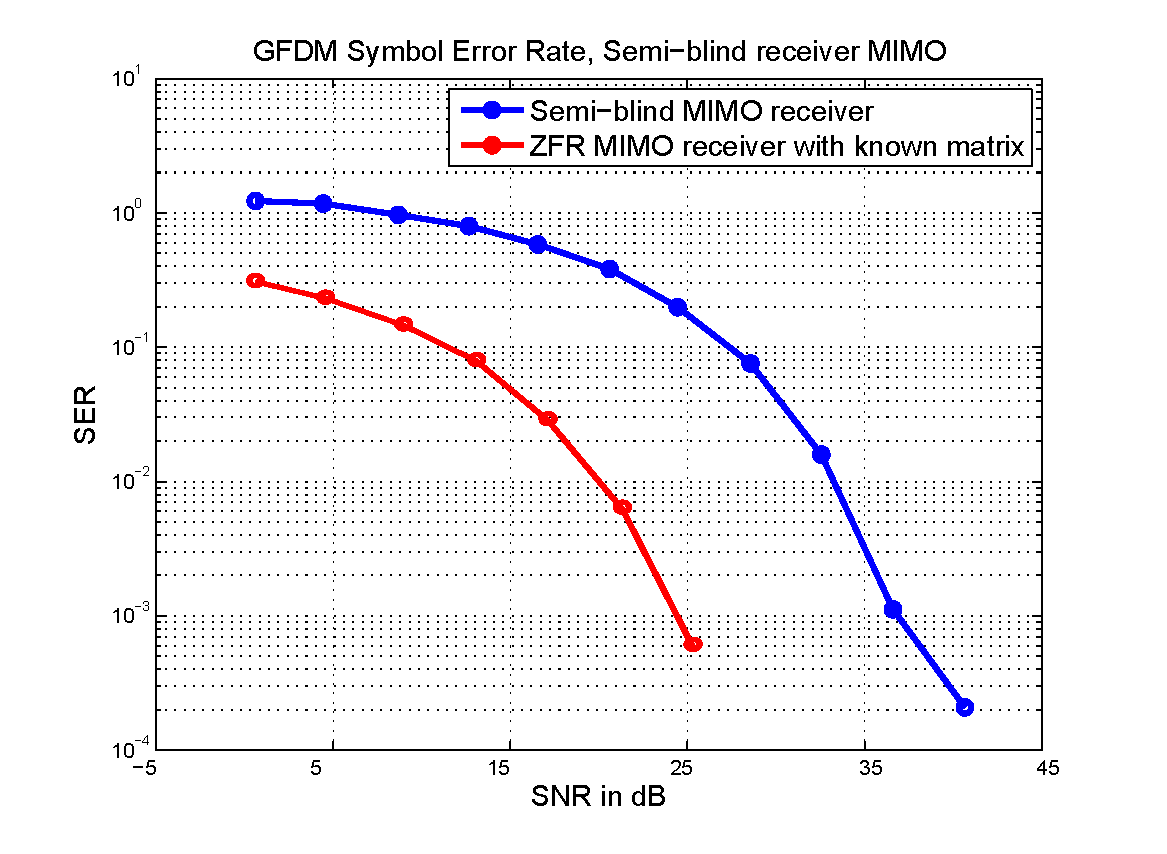
\includegraphics[width=0.9\columnwidth]{MIMO_SER_1.eps}
%\caption{\textit{\label{fs_m_0}SER for the channel orthogonalization in GFDM MIMO}}
%\end{figure}
\subsection{Scenario 2.1}
The performance results of the $\mathcal{A}$ search algorithm are obtained through simulation. The parameters of the system are tabulated in Table \ref{tab:m_table_1}.   
The GFDM system is simulated in the AWGN channel without coding. QPSK modulation scheme is used. The number of sub-carriers was $F=16$, samples for each symbol was $T/T_s=F$ The block size was $T_s=5$. The root-raised cosine filter was used with  roll-off factor $\alpha=0.5$. The selection coefficients was chosen mode two products between identity matrix in the first and third dimension with random integer values array.   The results of the GFDM performance is presented in the two plots, at first is shown the reconstruction error for the $\mathbf{A}$ fig. \ref{fig:fs_m_1}, at second is shown the SER in comparison with the case  if $\mathbf{a}=\mathbf{1}$ with the zero-forced receiver fig. \ref{fig:fs_m_2}. 
\begin{table}[H]
\caption{\label{tab:m_table_1}GFDM simulation parameters.Scenario 2.1}
\begin{center}
\begin{tabular}{|c|c|c|}
\hline
Parameter & Variable & GFDM \\
\hline
\hline
Transmit antennas &$M_t$&2 \\
\hline
Receive antennas &$M_r$&2 \\
\hline
Modulation scheme & $\mu$ & QPSK \\
\hline
Samples per symbol & $T/T_s$ & 16 \\
\hline
Sub-carriers&$F$&16 \\
\hline
Block size& $T_s$  &5 \\
\hline
Filter type&  &RRC \\
\hline
Roll-off-factor&$\alpha$  &0.5 \\
\hline
Sub-carrier coefficients& $\mathbf{a}_i$ & $unif(0,1)$ \\
\hline
Channel& $h$ &Flat-fading \\
\hline
Cyclic Prefix&  & No \\
\hline
Transmission&  & Uncoded\\
\hline
Decomposition rank& $rank$ & 25\\
\hline
\end{tabular}
\end{center}
\end{table}
\begin{figure}[H]
\centering
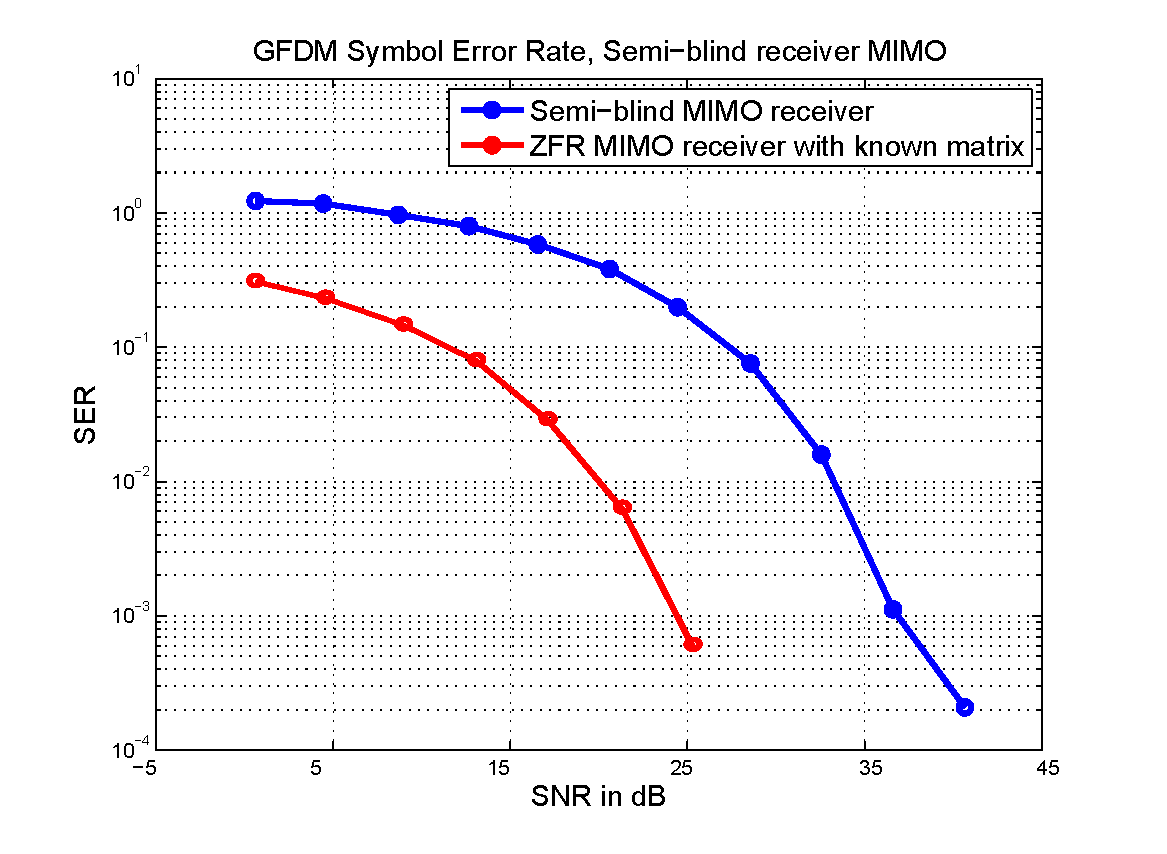
\includegraphics[width=0.9\columnwidth]{MIMO_SER_1.eps}
\caption{\label{fig:fs_m_1}\textit{SER dependency for the semi-blind MIMO receiver and ZF receiver with known channel}}
\end{figure}
\begin{figure}[H]
\centering
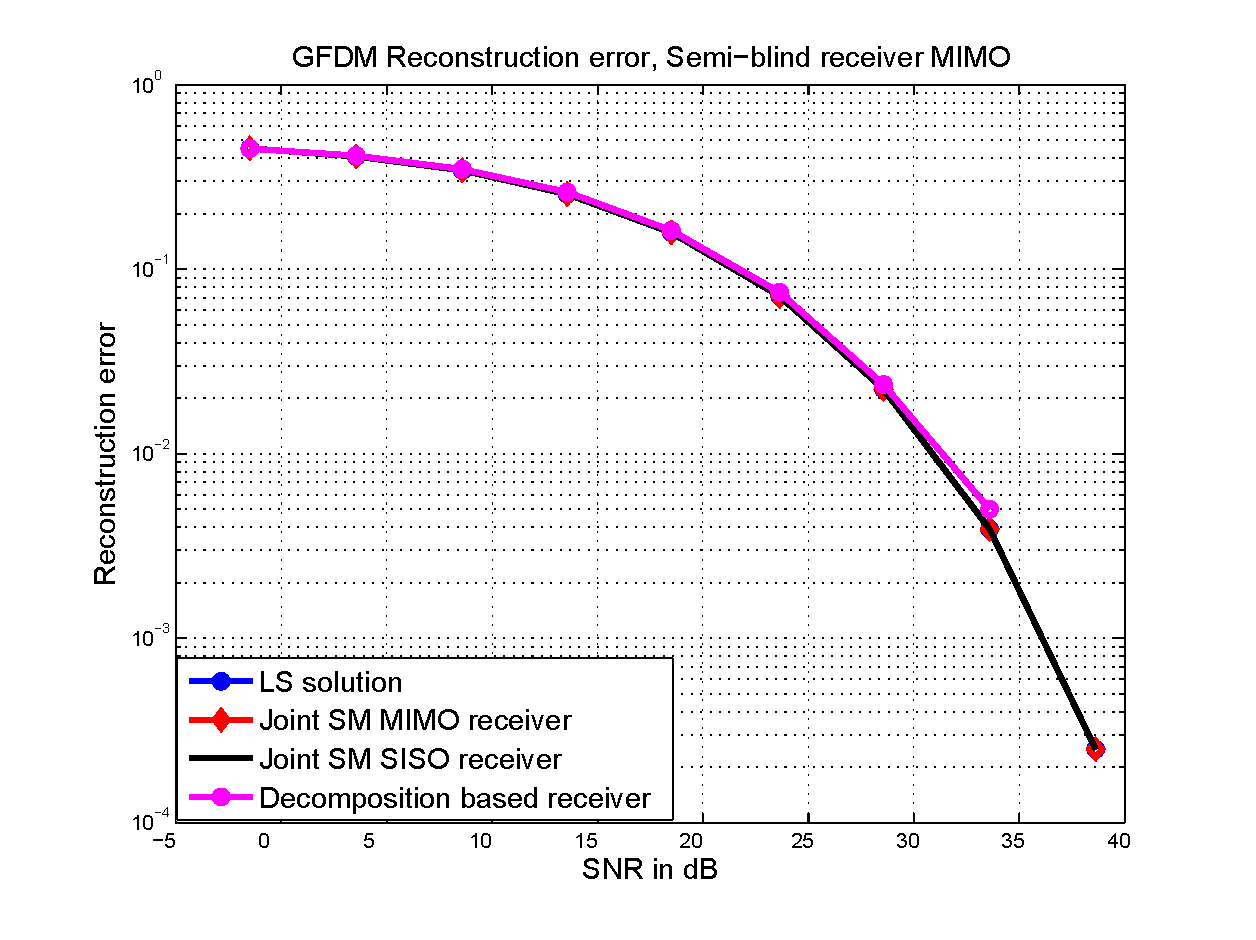
\includegraphics[width=0.9\columnwidth]{SM_RE_MIMO.eps}
\caption{\label{fig:fs_m_2}\textit{Reconstruction error for the sub-carrier estimation approaches}}
\end{figure}
\subsection{Scenario 2.2}
 \begin{table}[H]
\caption{\label{tab:m_table3}GFDM simulation parameters.Scenario 2.2}
\begin{center}
\begin{tabular}{|c|c|c|}
\hline
Parameter & Variable & GFDM \\
\hline
\hline
Modulation scheme & $\mu$ & QPSK \\
\hline
Samples per symbol & $T/T_s$ & 16 \\
\hline
Sub-carriers&$F$&16 \\
\hline
Block size& $T_s$  &5 \\
\hline
Transmit antennas &$M_t$&2 \\
\hline
Receive antennas &$M_r$&2 \\
\hline
Filter type&  &RRC \\
\hline
Roll-off-factor&$\alpha$  &1 \\
\hline
Length of the channel& $L+1$ & 12 \\
\hline
Channel& $h$ & Ped-A \\
\hline
Cyclic Prefix&  & No \\
\hline
Transmission&  & Uncoded\\
\hline
\end{tabular}
\end{center}
\end{table}
The GFDM system semi-blind receiver in the MIMO system is simulated in the frequency selective channel without coding. QPSK modulation scheme is used. The channel was generated in the two steps. At the first step was generated flat frequency channel matrix $\mathbf{H}$ with zero-mean circularly symmetric complex Gaussian random values. At the second step for each values of the matrix $\mathbf{H}$ generated the tensor $\mathcal{H}$ with time filter coefficients for each transmission link. At the end each slice of the tensor $\mathcal{H}$ is element-wise multiplied with $\mathbf{H}$. The number of the receive and transmit antennas was $M_r=M_t=3$.  The number of sub-carriers was $F=8$, samples for each symbol was $T/T_s=F$ The block size was $T_s=3$. The root-raised cosine filter was used with roll-of-factor $\alpha=1$. The length of the channel equal to $L+1=4$. The experiment setup is presented in the table \ref{tab:m_table3}. The results of the GFDM performance is presented in the two plots, at first \eqref{fig:fs_m_3} is shown the SER in comparison with the case  if receiver know the original channel and use the Zero-Forced receiver and with case for different number of unknown symbols in one transmission block. At second figure \eqref{fig:fs_m_4} is shown the reconstruction error for the channel values \eqref{sim:eq_m_1}.\begin{align}
R_e=\frac{\mid\mid\mathbf{A-\widehat{A}}\mid\mid^2}{\mid\mid\mathbf{A}\mid\mid^@}
\label{sim:eq_m_1}
\end{align}
\begin{figure}[H]
\centering
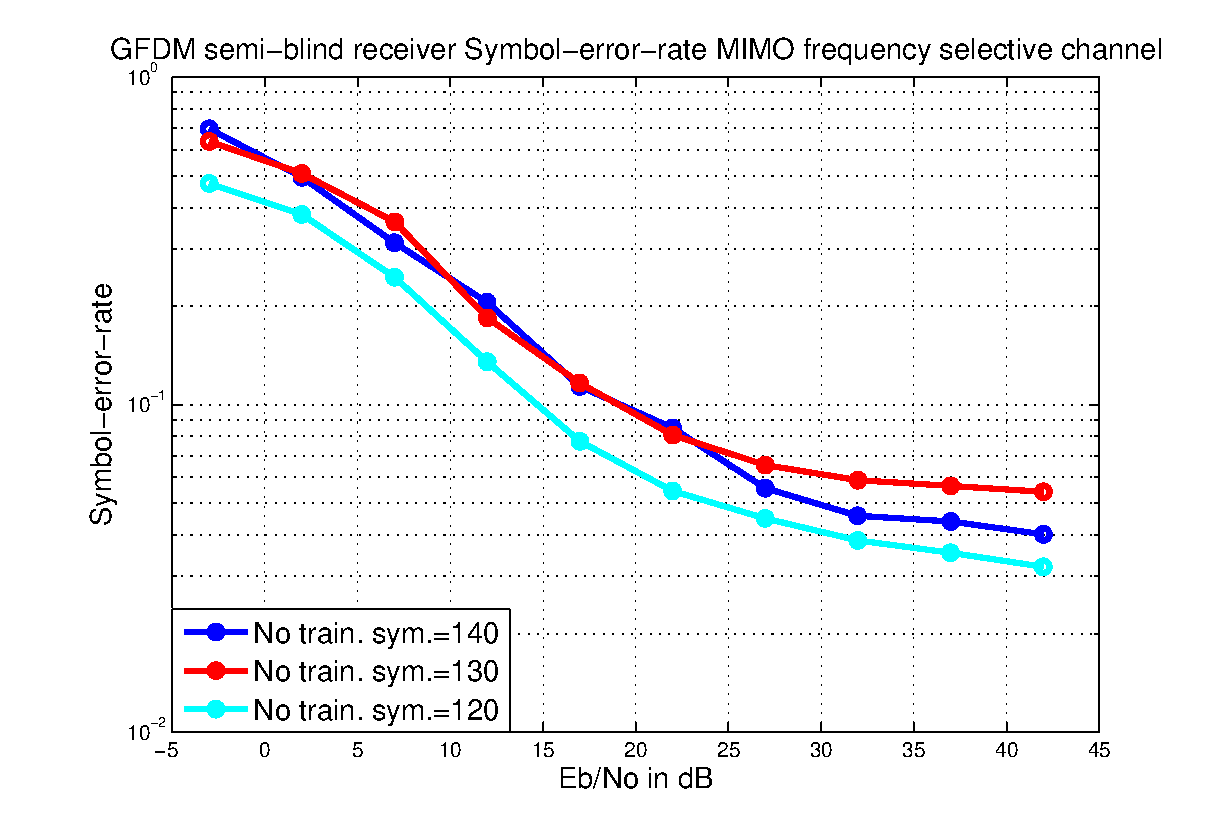
\includegraphics[width=0.9\columnwidth]{SM_MIMO_SER_ALS.eps}
\caption{\textit{SER for the semi-blind MIMO receiver with different number of known symbols}}
\label{fig:fs_m_3}
\end{figure}
\begin{figure}[H]
\centering
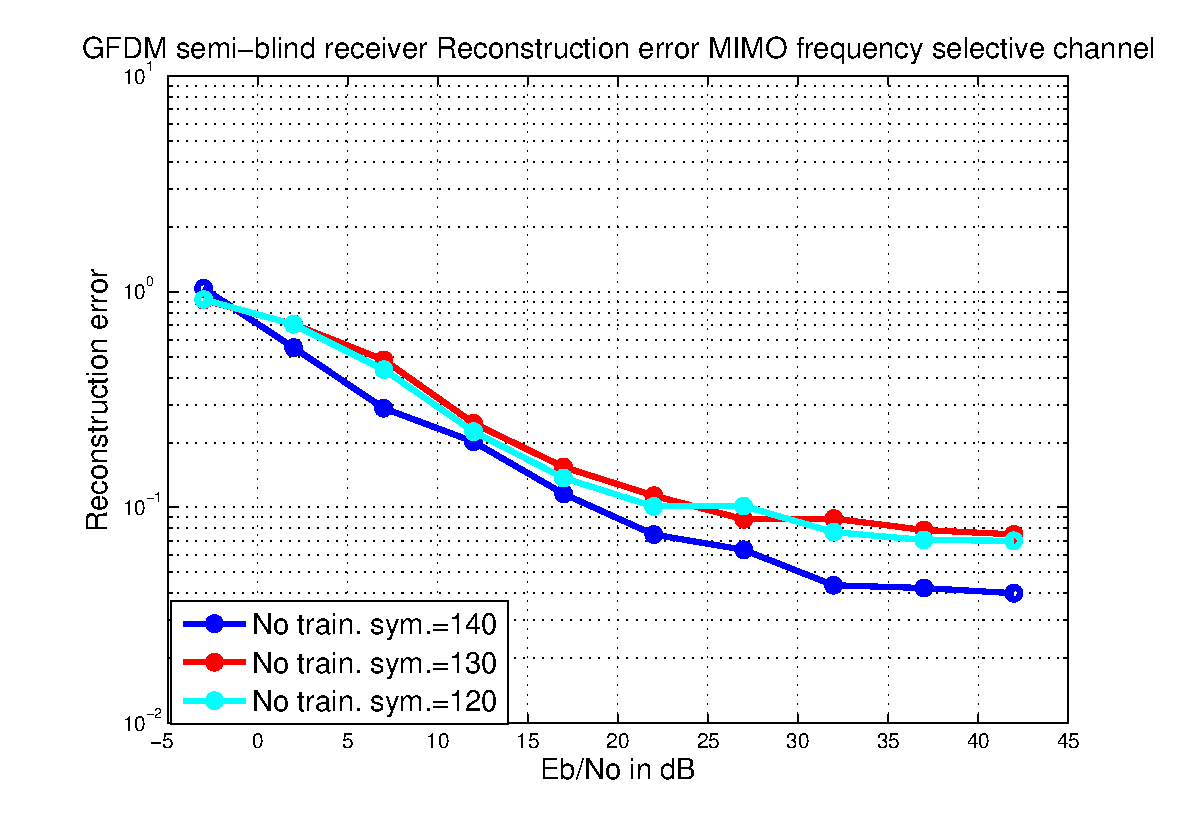
\includegraphics[width=0.9\columnwidth]{SM_MIMO_RE_ALS.eps}
\caption{\textit{Channel reconstruction error for the semi-blind MIMO receiver with different number of known symbols}}
\label{fig:fs_m_4}
\end{figure}
\subsection{Scenario 2.3}
The GFDM system Newton based semi-blind receiver in the MIMO system is simulated in the frequency selective channel without coding. QPSK modulation scheme is used. The channel was generated in the two steps. At the first step was generated flat frequency channel matrix $\mathbf{H}$ with zero-mean circularly symmetric complex Gaussian random values. At the second step for each values of the matrix $\mathbf{H}$ generated the tensor $\mathcal{H}$ with time filter coefficients for each transmission link. At the end each slice of the tensor $\mathcal{H}$ is element-wise multiplied with $\mathbf{H}$. The number of the receive and transmit antennas was $M_r=M_t=3$.  The number of sub-carriers was $F=8$, samples for each symbol was $T/T_s=F$ The block size was $T_s=3$. The root-raised cosine filter was used with roll-of-factor $\alpha=1$. The length of the channel equal to $L+1=4$. The experiment setup is presented in the table \ref{tab:m_table3}. The results of the GFDM performance is presented in the two plots, at first \eqref{fig:fs_m_5} is shown the SER in comparison with the case  if receiver know the original channel and use the Zero-Forced receiver and with case for different number of unknown symbols in one transmission block. At second figure \eqref{fig:fs_m_6} is shown the reconstruction error for the channel values. The reconstruction error is defined in the \eqref{sim:eq_m_2}
\begin{align}
R_e=\frac{\mid\mid\mathbf{h-\widehat{h}}\mid\mid^2}{\mid\mid\mathbf{h}\mid\mid^@}
\label{sim:eq_m_2}
\end{align}
\begin{figure}[H]
\centering
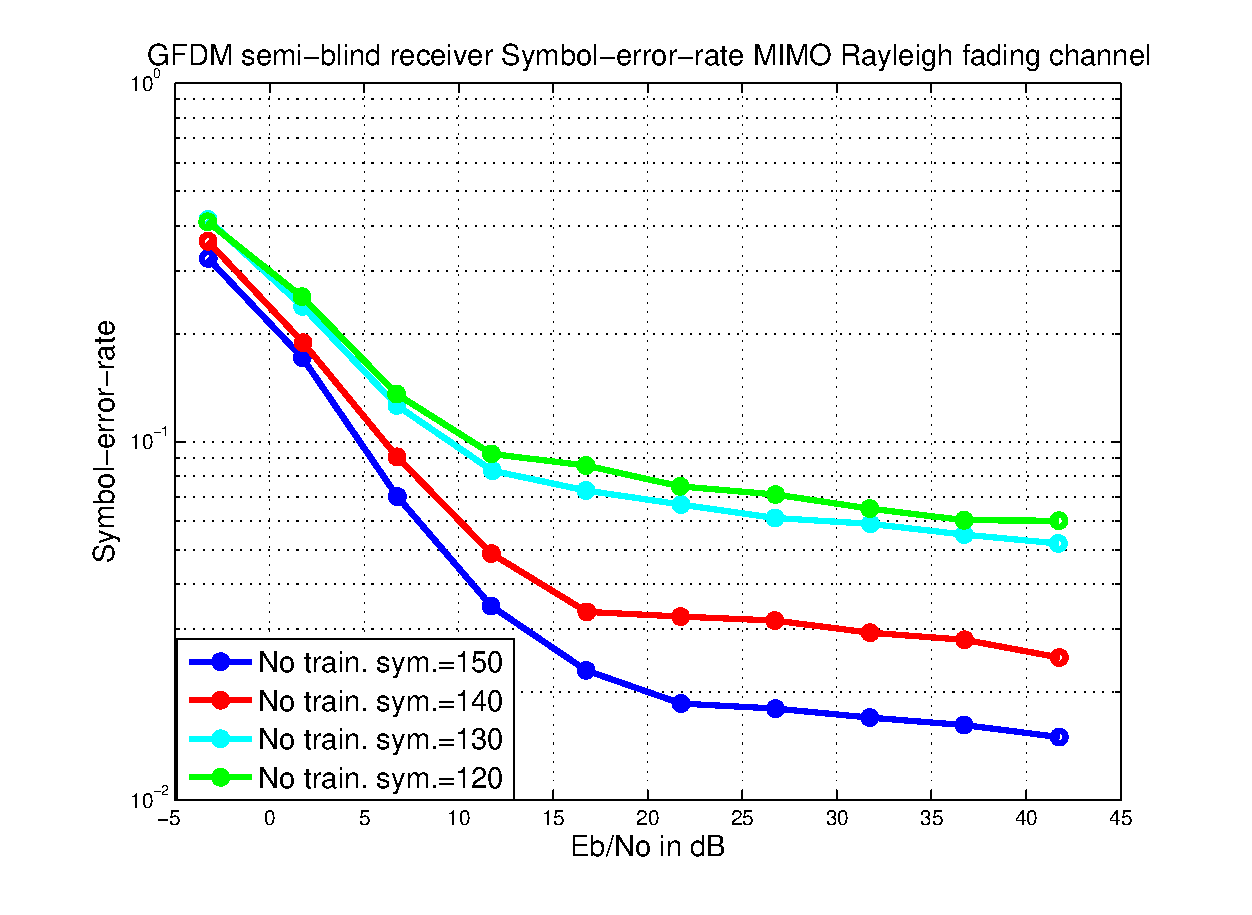
\includegraphics[width=0.9\columnwidth]{SM_MIMO_SER_N.eps}
\caption{\textit{SER for the semi-blind MIMO receiver with different number of known symbols}}
\label{fig:fs_m_5}
\end{figure}
\begin{figure}[H]
\centering
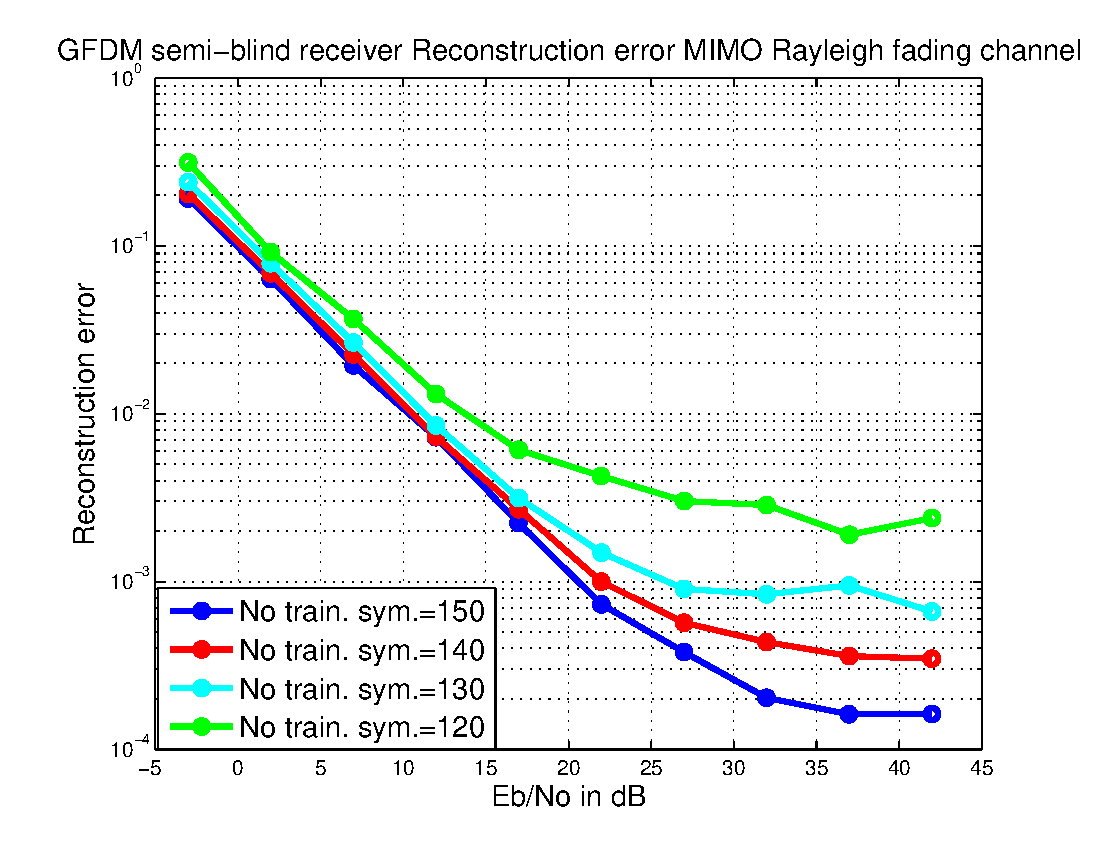
\includegraphics[width=0.9\columnwidth]{SM_MIMO_RE_N.eps}
\caption{\textit{Channel reconstruction error for the semi-blind MIMO receiver with different number of known symbols}}
\label{fig:fs_m_6}
\end{figure}
\section{Conclusion}\label{sec:CMIMO}

As conclusion for the second experiment with frequency coefficient selection approach in the MIMO case, we can see that algorithm decrease performance for 5-6 dB in comparison with system where the frequency coefficients known fig. \ref{fig:fs_m_2}. Decrease in performance come from the non-convenient coefficient selection way. The coefficients were chosen as $1$ if the resulting $abs(a_1)$ value is higher that $0.5$. There are better solutions to increase performance of the algorithm with the predefined information at the receiver.

We explained three frequency coefficients estimation approaches. As we can see from the result at the fig.\ref{fig:fs_m_3} all of them has the same result. Even the approximated solution based on the SISO model show the same performance. Due to that fact there is no difference with algorithm to choose. It should be noted that the joint MIMO algorithm allow to also the symbol estimation. Other algorithms can't estimate the symbols in the received data and work only if transmission block equal to the number of symbols in each subcarrier. There is one additional disadvantage of the Decomposition based approach, which doesn't converge with some initial points. Due to that fact decomposition based approach is less reliable than other algorithms.  The overall conclusion over the frequency selection coefficient algorithms we can say that spectrum sensing approach is applicable in the  MIMO case too. The system may use different subcarrier antennas for each transmit antenna and the receiver can estimate them. The performance loss is similar to the SISO case, but number of the time-slots decrease significantly in comparison with the SISO case. In the paper is explained very simple approaches to coefficients estimation.  Performance of the algorithm can be implemented in more efficient way without huge performance loss. We doesn't use any pre-processing and post-processing steps to increase performance.
 
%The main assumption of the SISO semi-blind based approach is error spread between transmit antennas. We ignored unknown values because unknown symbols at the receiver doesn't used. Repetition of the algorithm for the each transmit antenna allow to estimate coefficients for the sub-carrier selection matrix. Assumption is not applied for the time slots due to the overlapping and the receiver estimates the coefficient approximately. The error depends from the difference between sub-carrier selection coefficients in the each transmit antenna due to the time slot mixing in the GFDM systems. The SISO semi-blind based approach is the most expensive algorithm in comparison with others. The receiver can estimate parallel solution for the each sub-carrier selection coefficient corresponding to the each transmit antenna. The parallel solution decreases iteration time of the approach.
%The algorithm based on the least squares solution achieve the better results. The approach doesn't have assumptions in the mathematical model  for the GFDM system. But the least squares solution is very sensitive to the condition number of the matrix. The least squares solution is expensive too.
%The decomposition based approach of the unfolding multiplication with the matrix decrease size of the problem.  There is trade of between complexity of the task and calculation of the optimization process. Each iteration contain the matrix inversion inside. The matrix to invert change every iteration change from iteration to iteration.
%We can see that result of the all three algorithms is the same. There is significant difference for the decomposition based approach if we use the mean value metric. because we can choose bas initial point. Therefore we used the median value metric.

Next experiment is the semi-blind receiver channel and the symbol estimation over frequency selective channel with Rayleigh fading. The pedestrian-A channel was assumed in the each of the antennas. The experiment was done for the number of possible known symbols which have solution for the problem statement. The result for the SER if shown in the fig. \ref{fig:fs_m_3}. We can see from the plot, that performance of the algorithm is weak. With high SNR the algorithm has only $10^{-2}$ SER, which is very high value. This behavior is explained with the very bad conditioning of the channel matrix. The additional fact is the low performance of the Rayleigh fading channel itself. We can implement the more convenient ways of the algorithm to avoid such low performance. There is additional investigation about typical real channel should be done. We can see from the fig. the channel estimation has the upper bound of precision. We can say that algorithm has the same performance from the $30$ dB. There is significant dependency from the channel estimation precision as we can see here. The upper bound of the channel estimation doesn't allow increasing performance with higher SNR. As conclusion for the ALS based semi-blind receiver we can say that algorithm isn't provide full performance and they pre-processing and post-processing steps should be applied to increase the performance. This behavior will be investigated in the future work.
The last experiment show performance of the Newton based semi-blind receiver over the frequency selective Rayleigh fading channel. The fig.\eqref{fig:fs_m_5} show the performance of the algorithm in the symbol estimation. As we can see here the algorithm has the upper bound in the performance and doesn't allow to decrease the SER lower than $10^{-2}$. This behavior doesn't connect with error in the channel estimation, because the error in the channel estimation is upper bounded with much higher SNR and have precision near to the $10^{-3}$/ The main reason for this behavior is the high condition number of the Jacobian matrix. To implement the more precise and regularized solution the BFGS of Levenberg-Marquardt algorithm must be applied. We can see from the results, that there is significant dependency between the  number of the training symbols and performance of the system. The number of the training symbols is high due to the high number of estimated channel variables.The fig.\eqref{fig:fs_m_6} show the performance of the algorithm in the channel estimation. We can see that precision of the algorithm is high and algorithm estimates the channel with precision up to $10^{-3}$ reconstruction error. There are disadvantages of the algorithm which connected with bad conditioning and the computational complexity. The additional approaches must be investigated to overcome them. As conclusion for this algorithm we can propose two statements:
\begin{itemize}
\item Performance of the algorithm weak for the symbol estimation
\item Performance of the algorithm applicable for the channel estimation
\item The algorithm must use the regularizing approach.
\end{itemize}




%As we can see here, there is one optimal point in symbol estimation. The less unknown symbols in the block increase the SNR, whether the higher number of unknown symbols decrease performance of the approach. The solution where number of unknown symbols equal to $8$ show the closest result to the original GFDM system with the same block size, known channel and zero forced receiver. The channel reconstruction error has the similar behaviour and show the optimal point in the same number of unknown symbols. Important fact is that reconstruction error for the maximal and minimal number of unknown have different behaviour in comparison with the SISO model. But this behaviour also show the convexity of the performance function for the number of unknown symbols as variable. The different block size should have different optimal value of the unknown symbols, but the average performance must be the worse from the known channel system due to the higher energy per bit with same performance. 